% mnras_template.tex
%
% LaTeX template for creating an MNRAS paper
%
% v3.0 released 14 May 2015
% (version numbers match those of mnras.cls)
%
% Copyright (C) Royal Astronomical Society 2015
% Authors:
% Keith T. Smith (Royal Astronomical Society)

% Change log
%
% v3.0 May 2015
%    Renamed to match the new package name
%    Version number matches mnras.cls
%    A few minor tweaks to wording
% v1.0 September 2013
%    Beta testing only - never publicly released
%    First version: a simple (ish) template for creating an MNRAS paper

%%%%%%%%%%%%%%%%%%%%%%%%%%%%%%%%%%%%%%%%%%%%%%%%%%
% Basic setup. Most papers should leave these options alone.
\documentclass[a4paper,fleqn,usenatbib]{mnras}

% MNRAS is set in Times font. If you don't have this installed (most LaTeX
% installations will be fine) or prefer the old Computer Modern fonts, comment
% out the following line
\usepackage{newtxtext,newtxmath}
% Depending on your LaTeX fonts installation, you might get better results with one of these:
%\usepackage{mathptmx}
%\usepackage{txfonts}

% Use vector fonts, so it zooms properly in on-screen viewing software
% Don't change these lines unless you know what you are doing
\usepackage[T1]{fontenc}
\usepackage{ae,aecompl}


%%%%% AUTHORS - PLACE YOUR OWN PACKAGES HERE %%%%%

% Only include extra packages if you really need them. Common packages are:
\usepackage{graphicx}	% Including figure files
\usepackage{amsmath}	% Advanced maths commands
\usepackage{amssymb}	% Extra maths symbols
\usepackage{siunitx}

\usepackage{multirow}
\usepackage{lineno}
\linenumbers
%\usepackage{todonotes}

%%%%%%%%%%%%%%%%%%%%%%%%%%%%%%%%%%%%%%%%%%%%%%%%%%

%%%%% AUTHORS - PLACE YOUR OWN COMMANDS HERE %%%%%

% Please keep new commands to a minimum, and use \newcommand not \def to avoid
% overwriting existing commands. Example:
%\newcommand{\pcm}{\,cm$^{-2}$}	% per cm-squared

%%%%%%%%%%%%%%%%%%%%%%%%%%%%%%%%%%%%%%%%%%%%%%%%%%

%%%%%%%%%%%%%%%%%%% TITLE PAGE %%%%%%%%%%%%%%%%%%%

% Title of the paper, and the short title which is used in the headers.
% Keep the title short and informative.
\title[]{Evaluation of data compression techniques for the inference of
  stellar atmospheric parameters from high resolution spectra}

% The list of authors, and the short list which is used in the headers.
% If you need two or more lines of authors, add an extra line using \newauthor
\author[A. Gonz\'alez-Marcos et al.]{
A. Gonz\'alez-Marcos ,$^{1}$\thanks{Contact e-mail: \href{mailto:}{ana.gonzalez@unirioja.es}}
L. M. Sarro,$^{2}$
J. Ordieres-Mer\'e,$^{3}$
and A. Bello-Garc\'ia$^{4}$
\\
% List of institutions
$^{1}$ Department of Mechanical Engineering, University of La Rioja, c/ San Jos\'e de Calasanz, 31, 26004 Logro\~no, Spain  \\
$^{2}$ Dpto. de Inteligencia Artificial, ETSI Inform\'atica, UNED, c/ Juan del Rosal, 16, 28040 Madrid, Spain \\
$^{3}$ PMQ Research Team; ETSII; Universidad Polit\'ecnica de Madrid, Jos\'e Guti\'errez Abascal 2, 28016 Madrid, Spain\\
$^{4}$ Dept. of Construction and Industrial Manufacturing, University of Oviedo, 33203 Gij\'on, Spain\\
}

% These dates will be filled out by the publisher
\date{Accepted XXX. Received YYY; in original form ZZZ}

% Enter the current year, for the copyright statements etc.
\pubyear{2016}

% Don't change these lines
\begin{document}
\label{firstpage}
\pagerange{\pageref{firstpage}--\pageref{lastpage}}
\maketitle

% Abstract of the paper
\begin{abstract}
We evaluate the utility of several data compression techniques
  for alleviating the curse-of-dimensionality problem in regression
  tasks where the objective is to estimate stellar atmospheric
  parameters from high resolution spectra in the 4000-8000 K range. We
  conclude that Independent Component Analysis (ICA) performs better than the rest of the
  techniques evaluated for all compression ratios. We also assess the
  necessity to adapt the signal-to-noise ratio (SNR) of the training
  set examples to the SNR of each evaluation spectrum and conclude that
  within the conditions of our experiments, at most only two such models are
  needed (in the case of regression models for effective temperatures, 
  those corresponding to SNR=50 and 10) to cover the entire range. Finally, we also 
  compare the prediction accuracy of effective 
  temperature regression models for increasing values of the training grid 
  density and the same compression techniques. 
\end{abstract}

% Select between one and six entries from the list of approved keywords.
% Don't make up new ones.
\begin{keywords}
methods: statistical -- methods: data analysis -- stars: fundamental parameters -- methods: data compression
\end{keywords}

%%%%%%%%%%%%%%%%%%%%%%%%%%%%%%%%%%%%%%%%%%%%%%%%%%

%%%%%%%%%%%%%%%%% BODY OF PAPER %%%%%%%%%%%%%%%%%%

\section{Introduction}

The rapid evolution of astronomical instrumentation and the
implementation of extensive surveys have permitted the acquisition of
vast amounts of spectral data.  The reduction and management of large
spectral databases collected by large-area or all-sky surveys like
Gaia/Gaia-ESO \citep{2006MNRAS.367..290J,2012Msngr.147...25G}, RAVE
\citep{2006AJ....132.1645S}, or APOGEE \citep{2011AJ....142...72E}
require the use of automatic techniques for the consistent,
homogeneous, and efficient extraction of physical parameters from
spectra. The availability of these huge databases opens new
possibilities to better understand the stellar, Galactic, and
extra-galactic astrophysics. Of special importance is the
determination of intrinsic stellar physical parameters, such as
effective temperature ($T_{\rm eff}$), surface gravity (log
\textit{g}), metallicity ([M/H]) and alpha to iron ratio 
($\left[ \alpha/Fe \right]$). However, the difficulty that
atmospheric parameter estimation poses comes from the inherent size
and dimensionality of the data. {\bf That is, the number of measured
wavelengths in a single spectrum, which is the number of variables 
or dimensions of a dataset, is high as compared to the number of 
spectra or set of instances in the dataset. Thus,} regression from 
stellar spectra suffers the so-called {\sl curse of dimensionality} 
problem because the number of variables is much higher than the 
number of {\bf instances used to fit a regression model}. 
    
The \textit{curse of dimensionality} \citep{bellman:61} relates to 
the problem caused by the exponential increase in volume associated 
with adding extra dimensions to a mathematical space. 
{\bf When the number of data instances (set of spectra) is finite and 
the dimensionality (number of measured wavelengths in a single spectrum) 
increases, the volume of the space of independent variables increases so 
fast that it is not possible to ensure that there are several instances 
(spectra) with each combination of possible values that each dimension 
(measured wavelength) could have. That is, the density of data instances 
in the space decreases exponentially as the dimensionality increases. 
In other words, }
the available data become sparse. Because this sparsity is 
problematic for any method that requires statistical significance, the 
amount of data instances needed to support the result often grows 
exponentially with the dimensionality in order to obtain a statistically 
sound and reliable outcome.

Furthermore, typical spectra obtained in many surveys do not 
regularly reach the high signal-to-noise ratios (SNR) --about
100 or greater -- needed to obtain robust estimates, which
increases the difficulty to accurately estimate the physical
parameters of spectra.  In summary, stellar spectra are high
dimensional noisy vectors of real numbers and thus,
regression models must be both computationally efficient and robust
to noise.

There are several ways to alleviate this so-called \textit{curse of
  dimensionality}. It is evident that not all wavelength bins in an
observed spectrum carry the same amount of information about the
physical parameters of the stellar atmosphere. One way to reduce the
dimensionality of the space of independent variables is to concentrate
on certain wavelength ranges that contain spectral lines that are
sensitive to changes in the physical parameters. Before {\bf large-scale 
	spectroscopic surveys and the fast computers needed to analyse them 
	became available}, astronomers derived
physical parameters by interactively synthesizing spectra until a
subjective best fit of the observed spectrum in certain spectral lines
was found. But the number of spectra made available to the community
in the past decades have made this manual and subjective (thus
irreproducible) fitting procedure impractical. Automatic regression
techniques have therefore become a necessity.

The next step consisted in using derived features of the spectrum such
as fluxes, flux ratios or equivalent widths to infer the parameters
via multivariate regression techniques (see \citealt{2006ApJ...636..804A,
2010ApJ...720L.113R,2012ApJ...748...93R,2010MNRAS.405.1907B}; or \citealt{2006A&A...456.1109M}). 
That way, we significantly reduce the
full spectrum to a much smaller number of independent variables, at
the expense of introducing a feature extraction process: defining a
continuum level and normalizing the observed spectrum in the
wavelength region that contains the sensitive spectral feature. 
{\bf The normalization process effectively consists in dividing two 
	random variables: the observed flux and the estimated continuum 
	level. The simplest hypothesis consists in assuming that both 
	quantities are Gaussian distributed. Under these conditions, the normalized 
	spectrum will be a collection of random variables (one per 
	wavelength) each one distributed according to the ratio 
	distribution \citep[see e.g.][]{10.2307/2342070, 
		doi:10.1080/01621459.1965.10480783}. E}ven in the best case 
that the continuum flux is Gaussian distributed around a value significantly
different from zero, the ratio distribution is asymmetric {\bf (thus 
systematically biasing the result)} and has a heavy right tail 
{(\bf meaning that values significantly larger than the mode of the 
	distribution can occur with non-negligible probabilities)}. In the 
cases of low signal-to-noise spectra, the situation can be catastrophic.

The potential dangers associated with the feature extraction in
restricted wavelength ranges via continuum normalisation can be
mitigated by projecting the observed spectra onto bases of functions
spaces such as in the wavelet or Fourier decompositions 
(see \citealt{2010PASP..122..608M,2015MNRAS.452.1394L}; or 
\citealt{2015ApJS..218....3L}, for examples of the two approaches).
%\citep[see][for examples of the two approaches]{2010PASP..122..608M,2015MNRAS.452.1394L,2015ApJS..218....3L}.
{\bf In essence, the goal is to change the representation of the spectra,
originally involving a large number of variables (measured wavelengths),
into a low-dimensional description using only a small number of 
variables (dimensions). The new representation should preserve essentially 
all of the useful information within the high dimensional space.
Thus, by retaining only the most significant variables (dimensions) 
to represent the spectra, we achieve a data compression that can be 
of great benefit for estimating atmospheric parameters as it reduces 
the dimensionality of the space required to describe the data.}

The most popular data compression technique applied to stellar
spectra is Principal Component Analysis (PCA). It has been widely
applied in spectral classification combined with artificial neural
networks (ANN) \citep{singh:98} or support vector machines (SVM)
\citep{fiorentin:08b}. For continuum emission, PCA has a proven record
in representing the variation in the spectral properties of
galaxies. However, it does not perform well when reconstructing
high-frequency structure within a spectrum \citep{vanderplas:09}. To
overcome this difficulty, other methods have been used in the spectral
feature extraction procedure. Locally linear embedding (LLE)
\citep{roweisLLE:00} and Isometric feature map (Isomap)
\citep{tenenbaum:00} are two widely used nonlinear data
compression techniques. Some studies found that LLE is efficient in
classifying galaxy spectra \citep{vanderplas:09} and stellar spectra
\citep{daniel:11}. Other authors concluded that Isomap performs better
than PCA, except on spectra with low SNR (between 5 and 10)
\citep{bu:14}.

A detailed study of data compression techniques has to include the
analysis of their stability properties against noise. In order to
improve the overall generalisation performance of the atmospheric
parameters estimators, experience shows that it is advantageous to
match the noise properties of the synthetic training sample to that of
the real sample because it acts as a regulariser in the training phase
\citep{fiorentin:08a}.  The impact of the SNR on the parameter
estimation ($T_{\rm eff}$, log \textit{g} and [Fe/H]) with ANN 
is explored in \cite{snider:01}. They found
that reasonably accurate estimates can be obtained when networks are
trained with spectra --not derived parameters-- with similar SNR as
those of the unlabelled data, for {\bf SNR} as low as 13.

\cite{recio:06} determined three atmospheric parameters
($T_{\rm eff}$, log \textit{g} and [M/H]) and individual chemical
abundances from stellar spectra using the MATISSE (MATrix
Inversion for Spectral SynthEsis) algorithm. They introduced Gaussian
white noise to yield five values of SNR between 25 and 200 and found
that errors increased considerably for SNR lower than $\sim$ 25.  In
\cite{navarro:12} authors present a system based on ANN trained with
a set of line-strength indices selected among the spectral lines more
sensitive to temperature and the best luminosity tracers. They
generated spectra with a range of SNR between 6 and 200 by adding
Poissonian noise to each spectrum. Their scheme {\bf allows classification
of} spectra of SNR as low as 20 with an accuracy better than two spectral
subtypes. For SNR $\sim$ 10, classification is still possible but at a
lower precision.

In recent years, there seems to be a tendency to use {\bf the spectrum
rather than fluxes or equivalent widths derived from it} 
(see e.g. \citealt{2012ApJ...757..161T,2014A&A...567A...5R} and references therein; 
\citealt{2015ApJ...808...16N,2015MNRAS.448.2717W}; or \citealt{2015arXiv151000111R}). 
In this work we focus in this latter approach, and attempt to assess the
relative merits of various techniques to serve as a guide for future
applications of machine learning techniques for regression of stellar
atmospheric physical parameters.

This paper presents a comparative study of the most popular
data compression technique applied to stellar spectra (PCA)
and five alternatives (two linear and three nonlinear techniques). The
aims of the paper are (1) to investigate to what extent novel
data compression techniques outperform the traditional PCA on
stellar spectra datasets, (2) to test the robustness of these
techniques and their performance in atmospheric parameters estimation
for different SNRs, (3) to investigate the number of regression models
of different SNRs needed to obtain the best generalisation performance
for any reasonable SNR of the evaluation dataset, and (4) to analyse the effect
of the grid density over the regression performance in atmospheric
parameters estimation.  The investigation is performed by an empirical
evaluation of the selected techniques on specifically designed
synthetic datasets. In Sect. \ref{sec:dataset} we describe the datasets 
used in our experiments. In Sect. \ref{sec:dimred} we review the data compression
techniques evaluated in this work and their properties.  
Sect. \ref{sec:comparison1} presents our results when comparing the 
compression techniques and compression rates in terms of the atmospheric 
parameter estimation errors. In Sect. \ref{sec:comparison2} we evaluate 
the optimal match between the SNR of the training set examples to the SNR 
of the evaluation set, and in Sect. \ref{sec:comparison3} we present 
the main results from the analysis of the effect of the training set grid 
density over the regression performance. Finally, in Sect. 
\ref{sec:conclusions} we summarize the most relevant findings from 
the experiments and discuss their validity and limitations.

\section{The dataset}
\label{sec:dataset}

{\bf Spectra used in our experiments are divided into two groups:
\begin{itemize}
\item The training set, which refers to the portion of spectra used to 
	fit the atmospheric parameters models.
\item The evaluation set, which refers to that portion of the spectra 
	used only at the end of the model building to assess how well each 
	final model might perform on additional spectra.
\end{itemize}
}

The synthetic spectra that form the basis of our study have been
computed from MARCS model atmospheres \citep{gustafsson:08} and the
turbospectrum code \citep{alvarez:98, plez:12} together with atomic \&
molecular line lists. These spectra were kindly provided by the
Gaia-ESO team in charge of producing the physical parameters for the
survey \citep[see][for further details]{2012A&A...544A.126D}.
{\bf More specifically, our analyses were performed using spectra 
simulated with two different setups from the high-resolution (HR) 
mode of the GIRAFFE spectrograph, which was used to carry out the 
observations of the survey: the HR10 setup (534-562 nm) and the HR21 
setup (848-900 nm).}

The {\bf complete dataset (including training and evaluation data)} 
contains a grid of 8780 synthetic high-resolution spectra 
(\textit{R} = 19800) between 5339 and 5619 {\AA} (the nominal GIRAFFE 
HR10 setup) with effective temperatures between 4000 and 
8000 K (step 250 K), logarithmic surface gravities between 1.0 and 5.0 
(step 0.5), mean metallicities between -3.0 and 1.0 (with a variable step 
of 0.5 or 0.25 dex) and $\left[ \alpha/Fe \right]$ values varying between
-0.4 and +0.4 dex (step 0.2 dex) around the standard relation with the
following $\alpha$ enhancements: $\left[ \alpha/Fe \right]$ = +0.0 dex
for [M/H] $\geqslant$ 0, $\left[ \alpha/Fe \right]$ = +0.4 dex for
[M/H] = $\leqslant$ -1.0 and $\left[ \alpha/Fe \right]$ = -0.4[M/H]
for [M/H] between -1.0 and +0.0 (Fig.~\ref{fig:gridModelos}).
Elements considered to be $\alpha$-elements are O, Ne, Mg, Si, S, Ar,
Ca and Ti. The adopted solar abundances are those used by
\citep{gustafsson:08}. Fig.~\ref{fig:ejemplosEspectros} (left) shows some
example spectra from this dataset.   

\begin{figure}
	\centering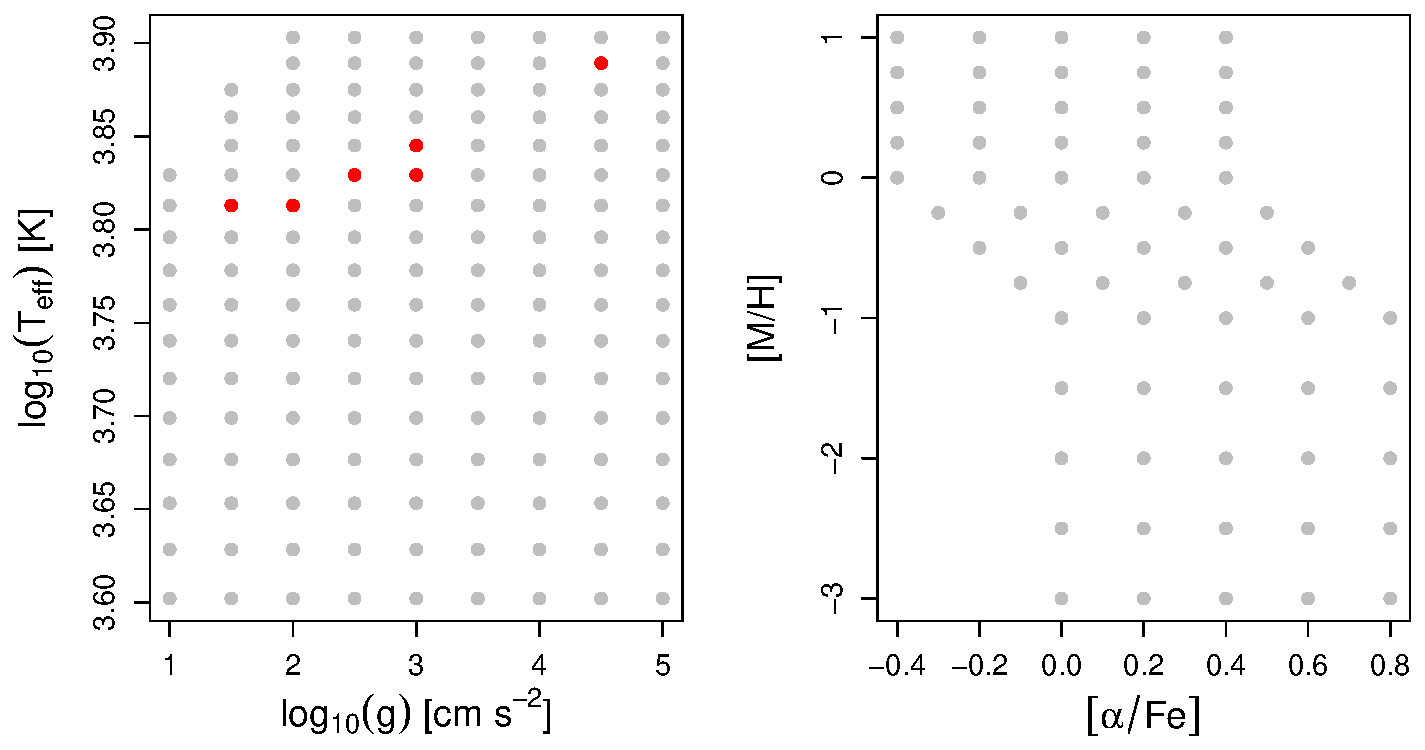
\includegraphics[width=\columnwidth]{fig01_grid_modelos.pdf}
	\caption{Coverage in parameter space of the dataset. Gray circles 
		represent spectra available in the original collection provided 
		by the Gaia-ESO collaboration. Red circles correspond to missing 
		spectra that were linearly interpolated as described in the text.}
	\label{fig:gridModelos}
\end{figure}

\begin{figure*}
	\centering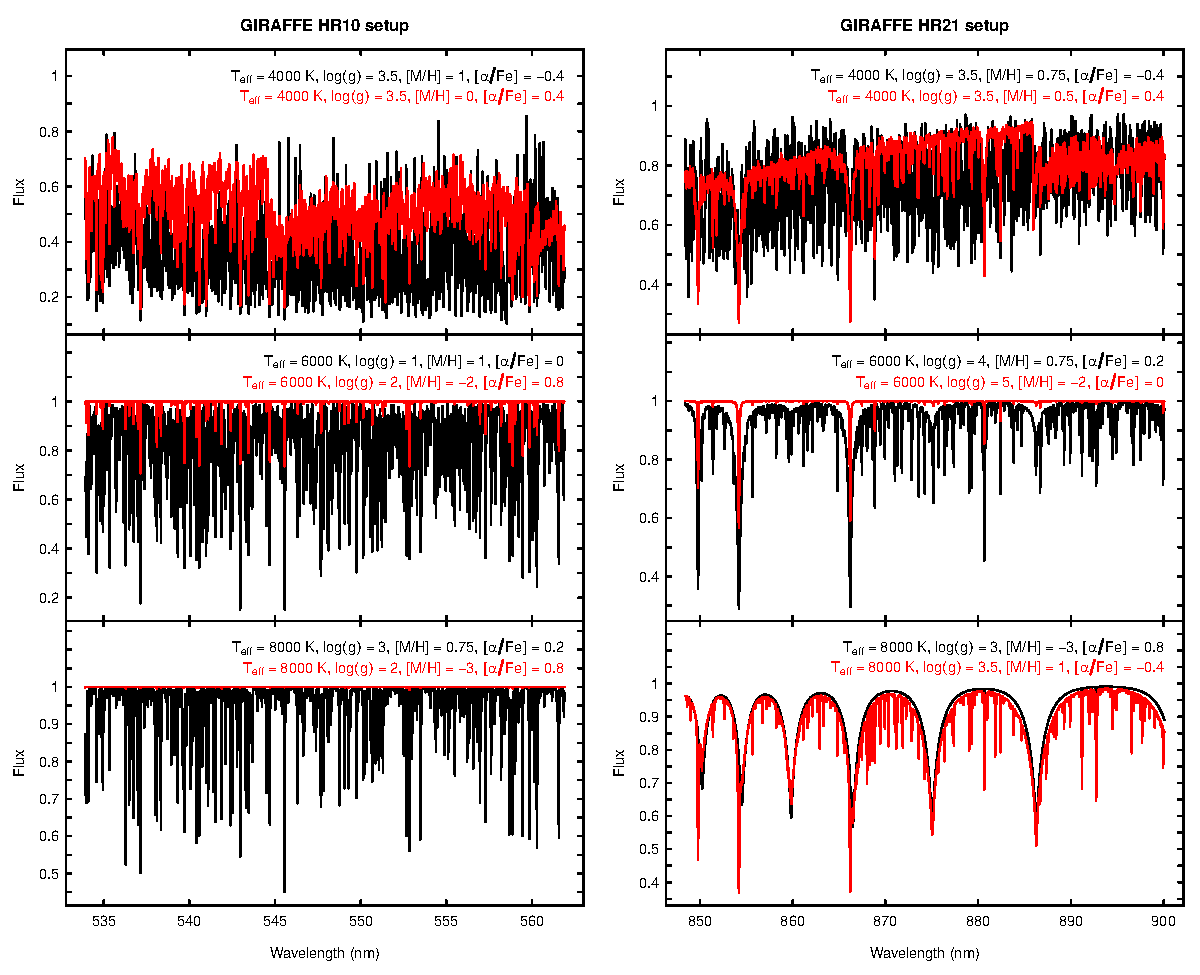
\includegraphics[width=\textwidth]{fig02_espectros_HR10_HR21.pdf}
	\caption{Example spectra from the nominal GIRAFFE 
		HR10 setup (left) and the nominal GIRAFFE HR21 setup (right).}
	\label{fig:ejemplosEspectros}
\end{figure*}

The sample size of our dataset (8780 spectra) is relatively
small compared to the input dimension (2798 flux measurements 
per spectrum). With the rule of thumb of a minimum of 10 samples per dimension  
	\citep{jain:00}, our dataset should contain at least $10^{2798}$ spectra.
In most real case applications in astronomy, the ratio of sample size to input 
dimensions is much lower and thus, the \textit{curse of dimensionality} 
problem is expected to affect even more severely the inference process. 

With a view to analyze the dependence of the validity of the results obtained 
with the selected dataset, we used a second dataset which is based on the same 
grid of atmospheric parameters but covering a different wavelength range. 
This new dataset contains high-resolution spectra (\textit{R} = 16200) between 
8484 and 9001 {\AA} (the nominal GIRAFFE HR21 setup). 
Fig.~\ref{fig:ejemplosEspectros} (right) shows some example spectra from 
this dataset. In this validity analysis, efforts were focused on the 
effective temperature.

\section{Data compression}
\label{sec:dimred}

{\bf In a dynamic environment, a complete rerun of a data compression 
algorithm becomes prohibitively time and memory consuming. 
For the sake of computational efficiency, the selection of the data
compression techniques tested in our experiments was done amongst those
capable of projecting new data onto the reduced dimensional space
defined by the training set without having to re-apply the algorithm
(process also known as out-of-sample extension).}
Thus, in this work, we investigated three linear data compression 
techniques such as PCA, independent component analysis (ICA) and 
discriminative locality alignment (DLA), as well as three nonlinear 
reduction techniques that {\bf can be generalised} to new data: wavelets,
Kernel PCA and diffusion maps (DM).  We aimed at minimizing the
regression error in estimating stellar atmospheric parameters with no
consideration of the physicality of the compression
coefficients. Physicality of the coefficients is sometimes required,
for example, when trying to interpret galactic spectra as a
combination of non-negative components{\bf, which closely resembles the
physical process of emission in the mid-infrared}.

Other linear and nonlinear techniques could be used for data
compression, such as linear discriminant analysis (LDA), locally linear
embedding (LLE), Isomap, etc. When the number of variables is much
higher than that of training samples, classical LDA cannot be directly
applied because all scatter matrices are singular and this method
requires the non-singularity of the scatter matrices involved.
Isomap's performance exceeds the performance of LLE, specially when
the data is sparse. However, in presence of noise or when the data is
sparsely sampled, short-circuit edges pose a threat to both Isomaps
and LLE algorithms \citep{saxena:04}. Short-circuit edges can lead to
low-dimensional embeddings that do not preserve a manifold's true
topology \citep{balasubramanianISOMAP:02}. Furthermore, Isomap and LLE
cannot be extended out-of-sample. 

%\begin{itemize}
%\item PCA. Linear, unsupervised
%\item ICA. Linear, unsupervised
%\item DLA. Linear, supervised
%\item Diffusion Maps. Non-linear, preserving global properties
%\item Wavelets. Non-linear, preserving global properties
%\item Kernel PCA. Non-linear, preserving global properties
%\end{itemize}

\subsection{Principal Component Analysis (PCA)}

PCA \citep{hotelling:33,pearson:01} is by far the most popular linear 
technique for data compression. The aim of the method is to reduce the
dimensionality of multivariate data whilst preserving as much of the
relevant information (assumed to be related to the variance in the
data) as possible. This is done by finding a linear basis of reduced
dimensionality for the data, in which the amount of variance in the
data is maximal. It is important to remark that PCA is based on the
assumption that variance is tantamount to relevance for the regression
task.

PCA transforms the original set of variables into a new set of
uncorrelated variables, the principal components, which are linear
combinations of the original variables. The new uncorrelated variables
are sorted in decreasing order of variance explained. The first
new variable shows the maximum amount of variance; the second
new variable contains the maximum amount of variation unexplained by
the first one, and is orthogonal to it, and so on.  This is
achieved by computing the covariance matrix for the full data
set. Next, the eigenvectors and eigenvalues of the covariance matrix
are computed, and sorted according to decreasing eigenvalue.

\subsection{Independent Component Analysis (ICA)}

ICA \citep{comon:94} is very closely related to the method called blind 
source separation (BSS) or blind signal separation \citep{jutten:91}. 
It is the identification and separation of mixtures of sources with 
little prior information. The goal of the method is to find a linear 
representation of non-Gaussian data so that the components are 
statistically independent, or as independent as possible \citep{hyvarinen:00}.

Several algorithms have been developed for performing ICA
\citep{bell:95,belouchrani:97,ollila:06,li:08}. A large widely used
one is the FastICA algorithm \citep{hyvarinen:00} which has a number
of desirable properties, including fast convergence, global
convergence for kurtosis-based contrasts, and the lack of any step
size parameter.  RobustICA \citep{zarzoso:10} represents a simple
modification of FastICA, and is based on the normalised kurtosis
contrast function, which is optimised by a computationally efficient
iterative technique. It is more robust than FastICA and has a very
high convergence speed.  Another widely used ICA algorithm is the
Joint Approximation Diagonalisation of Eigen-matrices (JADE)
\citep{cardoso:93}. This approach exploits the fourth-order moments in
order to separate the source signals from mixed signals. In this work
we selected the JADE algorithm for projecting the original spectra in
the space of independent components.

\subsection{Discriminative Locality Alignment (DLA)}
DLA \citep{zhang:2008} is a supervised manifold learning algorithm {\bf that 
performs data compression by utilizing the class label information of the 
data instances. A class is a collection of data instances with common 
characteristics and DLA uses this information to transform 
the dataset from a high dimensional space to a low dimensional space.
In our case, the values that each atmosphere parameter ($T_{\rm eff}$, 
log \textit{g}, [M/H] and $\left[ \alpha/Fe \right]$) could have are used 
as class labels. It is possible to apply this technique to our set of spectra 
because the number of possible values that each atmosphere parameter could 
have is limited.
}

The learning algorithm can be divided into three stages: part optimisation, 
sample weighting and whole alignment. In the first stage, {\bf for each 
spectrum a patch (region of the space of independent variables) is defined 
by the given spectrum and its nearest spectra based on a similarity (distance) 
measure.} On each patch, DLA preserves the local discriminative information 
through integrating the two criteria that {\textit{i}) the distances between 
intra-class spectra are as small as possible and \textit{ii}) the distance
  between the inter-class spectra is as large as possible. In the
  second stage, each part optimisation is weighted by the
  \textit{margin degree}, a measure of the importance of a given
  spectrum for classification. Finally, DLA integrates all the weighted
  part optimisations to form a global subspace structure through an
  alignment operation \citep{2002cs.......12008Z}. The projection
  matrix can be obtained by solving a standard eigendecomposition
  problem.
  
{\bf
DLA requires the selection of the following two parameters:
\begin{itemize}
\item Neighbour samples from an identical class ($k_1$): 
	the number of nearest spectra with respect to $x_i$
	from spectra in the same class with $x_i$
\item Neighbour samples from different classes ($k_2$): 
	the number of nearest spectra with respect to $x_i$
	from spectra in different classes with $x_i$
\end{itemize}
}
This method obtains robust classification performance under the
condition of small sample size. Furthermore, it does not need to
compute the inverse of a matrix, and thus it does not face the matrix
singularity problem that makes LDA and quadratic discriminant analysis 
(QDA) not directly applicable to stellar spectral data.

\subsection{Diffusion Maps (DM)}

DM \citep{coifman:06,nadler:06} are a non linear data compression 
technique for finding the feature representation of the datasets even 
if observed samples are non-uniformly distributed, {\bf i.e., the 
density of data instances (set of spectra in our case) in the space of 
independent variables is not uniform. The non-uniform data distribution 
leads to a reduction in the performance of an algorithm.

DM are based on the assumption that there exist a low-dimensional 
manifold or topological space embedded in the high-dimension space 
of independent variables. Thus, this technique aims to uncover the 
manifold structure in the data.
We conjecture that the spectra sharing the same atmospheric parameters 
must lie on some manifold. Therefore, we employ DM to discover the 
low-dimensional space that adequately represents such manifolds without
loss of information.
 
Graph representation is an effective mechanism to represent 
complex relationships between data points (spectra). Thus, the DM 
embedding begins with the construction of a graph. 
Each data point (spectrum) is represented by a collection of numerical 
variables (measured wavelenghts), and the condition for two nodes to be 
connected in the graph is based on the proximity of the corresponding 
data points (spectra) in the space of independent variables.
Subsequently, the data modeled as a graph is combined with Markov chain
techniques. In particular, random walks on the graph are used to obtain
a measure for the proximity of the data points (\textit{diffusion 
distance}), i.e., a measure of similarity between data points.
The remarkable idea is that eigenvectors of Markov matrices can be thought 
of as coordinates. Thus, the data, originally modeled as a graph, can be 
represented (embedded) as a cloud of points in a Euclidean space. 
The hope is that this new representation will capture the main structures 
of the data in a few dimensions.
In the low-dimensional representation of the data, DM attempt to retain 
the relationship between pairs of data points (spectra) as faithfully as 
possible.
}

%DM achieve data compression by re-organizing data according
%to parameters of its underlying geometry. DM are based on defining a
%Markov random walk on the data. By performing the random walk for a
%number of time steps, a measure for the proximity of the data points
%is obtained (\textit{diffusion distance}). In the low-dimensional
%representation of the data, DM attempt to retain the pairwise
%diffusion distances as faithfully as possible (under a squared error
%criterion). The key idea behind the diffusion distance is that it is
%based on integrating over all paths through the graph. This makes the
%diffusion distance more robust to short-circuiting than, e.g., the
%geodesic distance that is employed in Isomap \citep{tenenbaum:00}.

In this work, the results were optimised by controlling the degree of
locality in the diffusion weight matrix (referred to below with 
the parameter name \textit{eps.val}).

Finally, the classical Nystr\"{o}m formula \citep{NIPS2000_1866} was used
to extend the diffusion coordinates computed on a subsample (the training 
set) to other spectra (the evaluation set).


\subsection{Wavelets}

Wavelets \citep{mallat:98} are a set of mathematical functions used to
approximate data and more complex functions by decomposing the signal
in a hybrid space that incorporates both the original space where the
data lie (which we will refer to as original space), and the
transformed frequency domain. In our case, the original space will be
the wavelength space, but in representing time series with wavelets
the original space would be the time axis. The wavelet transform is a
popular feature definition technique that has been developed to
improve the shortcomings of the Fourier transform. Wavelets are
considered better than Fourier analysis for modelling because they
maintain the original space information while including information
from the frequency domain.

Wavelets can be constructed from a function (named \textit{mother 
wavelet}), which is confined to a finite interval in the original
space. This function is used to generate a set of functions through
the operation of scaling and dilation applied to the mother
wavelet. The orthogonal or biorthogonal bases formed by this set
allows the decomposition of any given signal using inner products,
like in Fourier analysis. {\bf That is, wavelet and Fourier analyses
are similar in the sense that both of them break a signal down into its 
constituent parts for analysis. However, whereas the Fourier transform 
decomposes a signal into a series of sine waves of different 
frequencies, the wavelet transform decomposes the signal into 
its \textit{wavelets} (scaled and shifted versions of the \textit{mother 
wavelet)}.

In particular, wavelet transform breaks a spectrum into subsequences at
different resolution scales, i.e., it decomposes a spectrum at different 
dilations to obtain (\textit {i}) those approximation coefficients that 
represent the high-scale and low-frequency components of the spectrum and 
(\textit {ii}) the detail coefficients that represent the low-scale and 
high-frequency components of the spectrum. 
%At high frequency (shorter time intervals), the wavelets can capture 
%discontinuities, ruptures and singularities in the original spectrum. 
%At low frequency (longer time intervals), the wavelet characterizes the 
%coarse structure of the spectrum to identify the long-term trends. 
Thus,} wavelet analysis offers multi-resolution analysis 
in the original space and its frequency transformed domain, and it can be 
useful to reveal trends, breakdown points or discontinuities.

Data compression with wavelets consists of keeping a reduced
number of wavelet coefficients. There are two common ways of
coefficient selection: (\textit i) to eliminate the {\bf detail}
coefficients that are assumed to reflect only random noise, 
and (\textit {ii}) to keep the $k$ most statistically significant
wavelet coefficients (which yields a representation of the signal with
less variance) \citep{li:10}. There are more sophisticated ways to
further reduce the number of wavelet coefficients using standard machine
learning techniques for feature selection, such as the LASSO
(Least Absolute Shrinkage and Selection Operator) used in
\cite{2015MNRAS.452.1394L}, wrapper approaches, information theory
measures, etc. A full analysis of all these alternatives is out of
the scope of this paper and we will only apply the first reduction
mentioned above.

\subsection{Kernel PCA}

Kernel PCA is the reformulation of traditional linear PCA in a
high-dimensional space that is constructed using a kernel function
\citep{sholkopf:98}. This method computes the principal eigenvectors
of the kernel matrix, rather than those of the covariance matrix. The
reformulation of PCA in kernel space is straightforward, since a
kernel matrix is similar to the inner product of the datapoints in the
high-dimensional space that is constructed using the kernel function
(the so-called {\textit kernel trick}). The application of PCA in the
kernel space allows for the construction of nonlinear mappings of the
input space.

Since Kernel PCA is a kernel-based method, the mapping performed
relies on the choice of the kernel function. Possible choices for the
kernel function include the linear kernel (i.e., traditional PCA), the
polynomial kernel, and the Gaussian kernel. An important weakness of
Kernel PCA is that the size of the kernel matrix is proportional to
the square of the number of instances in the dataset.

In this work we used the Gaussian kernel and optimized the predictive
performance by fine tuning the inverse kernel width ($\sigma$). 

\section{Comparison of spectrum compression techniques and optimal rates}
\label{sec:comparison1}

We investigate the utility of six data compression techniques
for feature extraction with a view to improving the performance of
atmospheric parameters regression models. The robustness of these
techniques against increasing SNR is evaluated, and the generalisation
performance of training sets of varying SNRs is analysed.

Our set of experiments proceeds in three stages. In the first stage we
aim at comparing the various compression techniques and compression
rates {\bf for different SNR regimes} in terms of the atmospheric 
parameter estimation errors. As a result of these experiments, we select 
an optimal compression approach and rate (dimensionality of the reduced 
space).

Different machine learning models have been used for the automatic
estimation of atmospheric parameters from stellar spectra. Two of the
most widely used techniques in practice are ANN and support vector 
machines (SVM). Unlike ANN, SVM does not need
a choice of architecture before training, but there are some
parameters to adjust in the kernel functions of the SVM. We use SVM
with radial basis kernel functions and adjust the SVM parameters by
maximizing the quality of the atmospheric parameter ($T_{\rm eff}$,
log \textit{g}, [M/H] or $\left[ \alpha/Fe \right]$) prediction as 
measured by the root mean squared error (RMSE, Eq.~\ref{eq:rmse}) 
in out-of-sample validation experiments.

\begin{equation}
\label{eq:rmse}
RMSE_k=\sqrt{\frac{1}{n}\sum_{i=1}^{n}\left(\hat{\theta}_{k;i}-\theta_{k;i}\right)^{2}}
\end{equation}

where $k$ indexes the atmospheric parameter 
	(${\theta}_{k}$ is one of $T_{\rm eff}$, log \textit{g}, 
	[M/H] or $\left[ \alpha/Fe \right]$), $\hat{\theta}_{k;i}$ and $\theta_{k;i}$
	are the predicted and target values of ${\theta}_{k}$ for the $i$-th 
	sample spectrum, and $n$ represents the total number of spectra in our evaluation set.
  
{\bf In order to study the dependency of the estimation performance on the
noise level of the input spectra, Gaussian white noise of different
variances (SNRs equal to 100, 50, 25 and 10) was added to the original
synthetic spectra.} 
Then, the datasets were randomly split into two subsets, one for training
(66\% of the available spectra) and one for evaluation (the remaining
34\%). Since the goal of these first experiments is to compare the
compression techniques rather than obtaining the best predictor,
splitting the dataset into training and evaluation sets is considered
a good scheme. In essence, the experimental procedure consists of the
following steps illustrated in Fig.~ \ref{fig:flowchart}:

\begin{enumerate}
\item \label{itemone} Compute the low-dimensional representation of
  the data using the training set. Because some of the techniques used
  to reduce the dimensionality depend on the setting of one or more
  parameters, a tuning process was performed in order to determine the
  optimal parameter values (in the sense that minimize the RMSE; 
  see below). Table~\ref{tab:parameters} presents the ranges of 
  values that were searched, as well as the best parameter value
  obtained in each case.
\item \label{itemtwo} Construct SVM models using the training set, and a varying
  number of dimensions (2, 5, 10, 15, 20, 25, 30 and 40) of the
  reduced space. The SVM parameters (kernel size and soft-margin
  width) and the compression parameters (where applicable; see 
  Table~\ref{tab:parameters}) are fine-tuned to minimize the prediction error of the
  atmospheric parameter ($T_{\rm eff}$, log \textit{g}, [M/H] or 
  $\left[ \alpha/Fe \right]$).
\item \label{itemthree} Project the evaluation spectra onto the
  low-dimensional space computed in step \ref{itemone}.
\item Obtain atmospheric parameter predictions by applying the SVM
  models trained in step \ref{itemtwo} to the evaluation set obtained in
  step \ref{itemthree}.
\item Calculate the performance of the predictor based on the RMSE
  obtained on the evaluation set.
\end{enumerate}

\begin{figure*}
\centering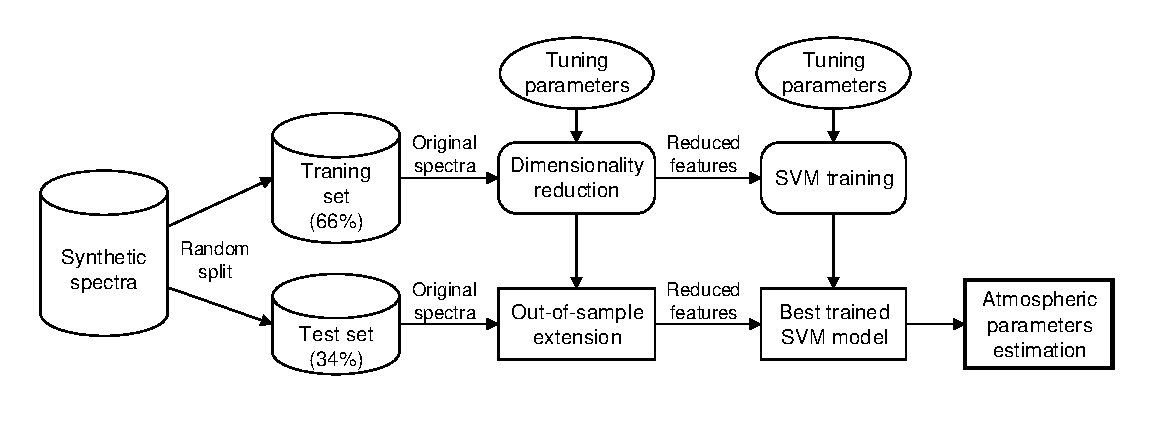
\includegraphics[width=0.85\textwidth]{flowchart.pdf}
\caption{Process flow chart for investigating the performance of the 
selected data compression techniques.}
\label{fig:flowchart}
\end{figure*}

\begin{table}
\centering
\caption{Summary of the parameters analysed for the 
data compression techniques.}
\label{tab:parameters}
\begin{tabular}{l c c c}
\hline
\multirow{2}{*}{\textbf{Technique}} & \multirow{2}{*}{\textbf{Parameter}} & \textbf{Analysed} &  \textbf{Best} \\
  	&   & \textbf{range} & \textbf{value} \\
\hline
\multirow{2}{*}{DLA} 
	& $k_1$ & [2 - 8]  & 2 \\\cline{2-4}
	& $k_2$ & [2 - 8]  & 3 \\\hline
DM & eps.val & [0.01 - 700] & 600 \\\hline
Kernel PCA & $\sigma$ & [0.0001 - 0.01] & 0.001 \\
\hline
\end{tabular}
\end{table}

\subsection{Results}

First, we compare the performance of the data compression
techniques described in section \ref{sec:dimred} using noise-free
synthetic spectra as well as degraded spectra with SNR levels of 100,
50, 25 and 10. Figures \ref{fig:02} to \ref{fig:07} show the RMSE
obtained with the evaluation set of the HR10 spectra (the 33\% 
of the full set of spectra that was not not used to define the 
compression transformation or to train SVM models) grouped by SNR. 
Equivalent figures grouped by compression technique are included in 
Appendix \ref{a1} to facilitate comparisons.

\begin{figure*}
\centering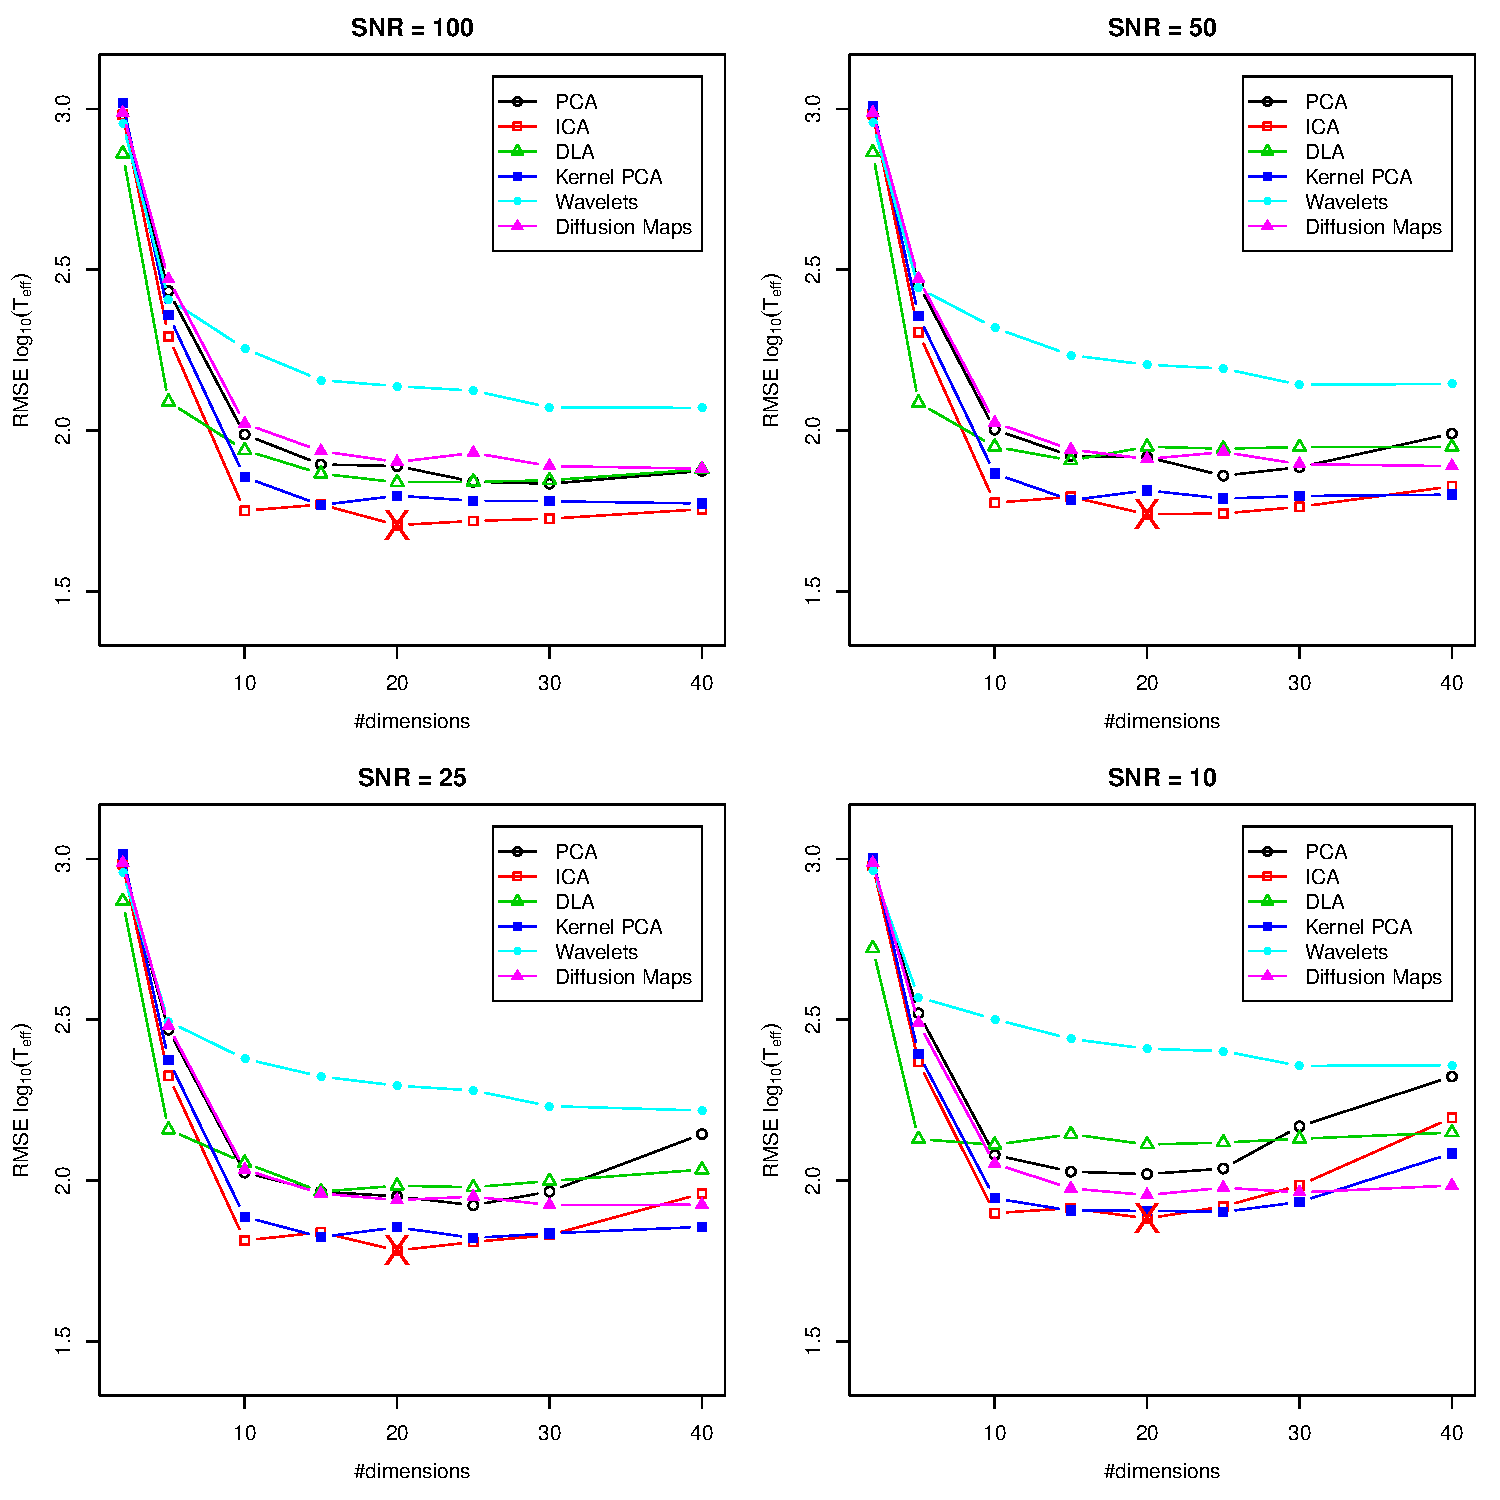
\includegraphics[width=\textwidth]{flamesHR10_Teff_log_BestSVM_N-RMSE_test.pdf}
\caption{Temperature estimation errors as a function of the number of
  dimensions used for data compression, for noisy synthetic
  spectra from the nominal GIRAFFE HR10 setup.}
\label{fig:02}
\end{figure*}

\begin{figure*}
\centering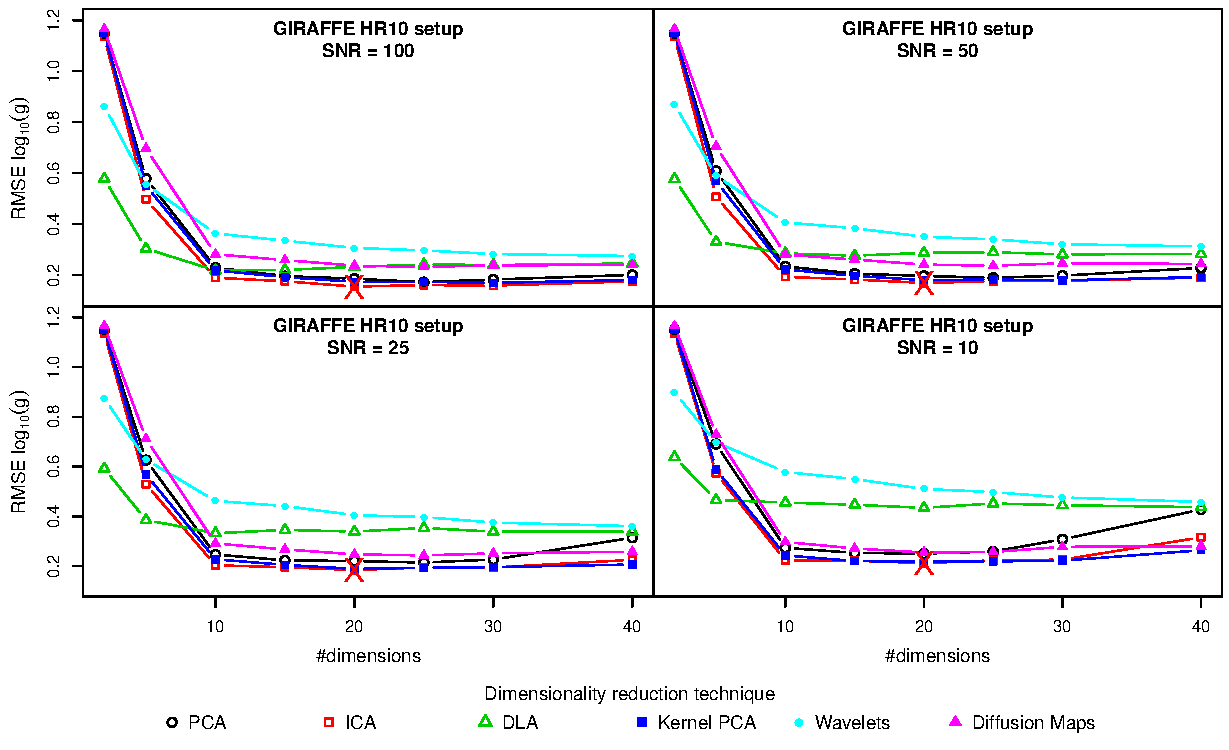
\includegraphics[width=\textwidth]{flamesHR10_Logg_BestSVM_N-RMSE_test.pdf}
\caption{Surface gravity estimation errors as a function of the number of
  dimensions used for data compression, for noisy synthetic
  spectra from the nominal GIRAFFE HR10 setup.}
\label{fig:04}
\end{figure*}

\begin{figure*}
\centering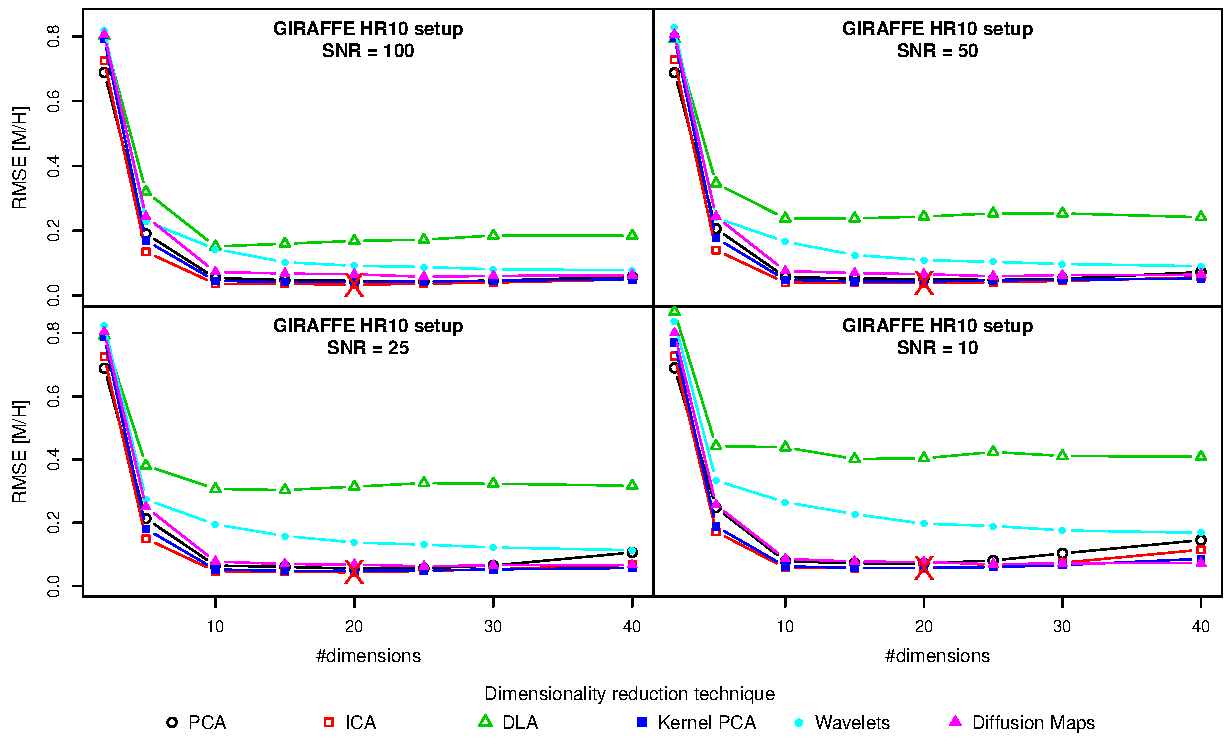
\includegraphics[width=\textwidth]{flamesHR10_Meta_BestSVM_N-RMSE_test.pdf}
\caption{Metallicity estimation errors as a function of the number of
  dimensions used for data compression, for noisy synthetic
  spectra from the nominal GIRAFFE HR10 setup.}
\label{fig:06}
\end{figure*}

\begin{figure*}
\centering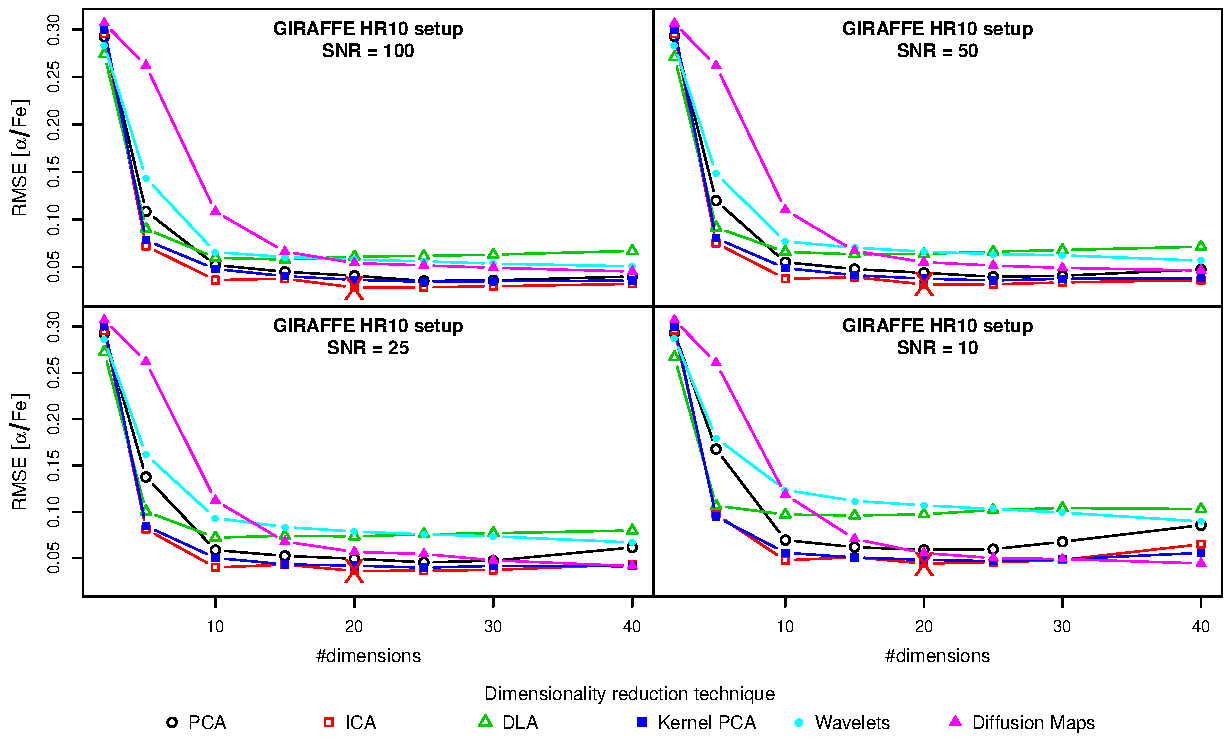
\includegraphics[width=\textwidth]{flamesHR10_AlFe_BestSVM_N-RMSE_test.pdf}
\caption{$\left[ \alpha/Fe \right]$ estimation errors as a function of the number of
  dimensions used for data compression, for noisy synthetic
  spectra from the nominal GIRAFFE HR10 setup.}
\label{fig:07}
\end{figure*}

Inspection of the figures reveals that the best strategies to compress
the spectra are kernel PCA and ICA, with ICA performing marginally 
better than kernel PCA in most of the parameter space, except sometimes for the lowest
compression rate. RMSE errors increase only moderately down to a SNR
of 10, which seems to indicate that most of the examined compression
techniques serve well as noise filters.

The performance comparison of the analysed data compression
techniques shows that although traditional PCA is not the most
efficient method, it outperforms some of the nonlinear techniques used
in this study, such as DM or wavelets. %{\bf We need to propose an explanation}. 
The lower performance of DM compared to that of PCA  could be partially explained by the 
Nystr\"{o}m extension. Although this method results in diffusion coordinates 
very similar to those that would be obtained by including the new spectra in 
the diffusion map, it may lead to small losses of 
prediction accuracy. As an illustration, the RMSE obtained for the 
$T_{\rm eff}$ in the high SNR regime (SNR=100) is between {0.5}--{1.5}\% 
better if the diffusion coordinates were computed 
from the whole dataset, instead of applying the out-of-sample extension.
In the case of wavelets, it seems clear that even at the lowest 
compression rates of 40 components we are eliminating
spectral information that is relevant for the subsequent regression task. 

Overall, wavelets combined with SVM models have the highest errors
regardless of the number of retained dimensions, with the exception of
the [M/H] estimation where DLA performed worse for noisy synthetic
spectra. Then, DLA was outperformed by most other techniques (except wavelet 
compression) for almost any compression rate and SNR. However, 
it achieved the lowest prediction errors for the hardly useful scenarios of noise-free data 
(not shown here for the sake of conciseness) or the highest compression 
rates (two or five dimensions) when estimating $T_{\rm eff}$ and 
log \textit{g}. PCA and DM yield similar $T_{\rm eff}$ prediction
errors in the high SNR regime, but DM are more robust against noise
specially for the lowest compression rates examined.

It is interesting to note that compression techniques can be grouped
into two categories: DLA, DM and Wavelets show a flat RMSE for target
dimensions greater than ten, even for the lowest SNR explored in this
Section (SNR=10); PCA, Kernel PCA and ICA show positive slopes in the
RMSE curves for SNRs below 25 and target dimensionalities greater than
25, indicating that components beyond this limit are increasingly
sensitive to noise. 

The relative difference of DM with respect to the best
performing compression techniques (ICA and kernel PCA) improves as the
SNR diminishes until it becomes almost comparable for SNR=10, while at
the same time rendering the SVM regression module insensitive to the
introduction of irrelevant features (as shown by the flat RMSE curves
for increasing numbers of dimensions used). 

Table~\ref{tab:01} quantifies the prediction errors of the best models
for each SNR. It is interesting that ICA compression with 20
independent components remains as the best option for any SNR, except
for the unrealistic noise-free data. 
These results evidence that for a given sample
size (the number of spectra in the training set) there is
an optimal number of features beyond which the performance of the
predictor will degrade rather than improve. On the other hand, as
expected, the quality of atmospheric parameter predictions degrades 
for lower SNR. However, RMSE errors were relatively low even for 
low SNR ($\sim$ 10).  

\begin{table*}
\centering
\caption{RMSE on the evaluation set of 2986 spectra for the best SVM trained models (HR10).}
\label{tab:01}
%\resizebox{0.99\textwidth}{!}{%
\begin{tabular}{l c c c c c c}
\hline
\multirow{2}{*}{\textbf{SNR}} & \multirow{2}{*}{\textbf{Method}} & \multirow{2}{*}{\textbf{Nr. Dim.}} & {\bf RMSE} & {\bf RMSE} & {\bf RMSE} & {\bf RMSE}\\
 &  &  & \textbf{$T_{\rm eff}$ (K)} & \textbf{log \textit{g}} & \textbf{[M/H] (dex)}  & \textbf{$\left[ \alpha/Fe \right]$ (dex)}\\
\hline
$\infty$ & DLA / ICA\protect\footnotemark[1] & 40 / 30 / 20\protect\footnotemark[2] & 27.16 & 0.13 & 0.017 & 0.025\\
100 & ICA & 20 & 50.81 & 0.15 & 0.033 & 0.028\\
50 & ICA & 20 & 54.91 & 0.17 & 0.038 & 0.032\\
25 & ICA & 20 & 60.59 & 0.18 & 0.043 & 0.036\\
10 & ICA & 20 & 76.21 & 0.21 & 0.057 & 0.044\\
\hline
\multicolumn{7}{l}{\textsuperscript{1}\footnotesize{The best performance for $T_{\rm eff}$, log 
		\textit{g} and [M/H] was obtained with DLA,  while best}}\\
\multicolumn{7}{l}{\footnotesize{performance for $\left[ \alpha/Fe \right]$ was obtained with ICA.}}\\
\multicolumn{7}{l}{\textsuperscript{2}\footnotesize{The best performance for $T_{\rm eff}$ and log 
		\textit{g} was obtained with 40 dimensions, while for [M/H] and}}\\ 
		\multicolumn{7}{l}{\footnotesize{ 
		$\left[ \alpha/Fe \right]$, 30 and 20 dimensions were needed respectively.}}
\end{tabular}
%}
\end{table*}

%%%%%%%%%%%%%%%%%%%%%%%%%%%%%%%%%%%%%%%%%%%%%%%
%%% HR21
\subsubsection{Applicability of the HR10 results to the HR21 setup}

The same analysis was carried out on the HR21 dataset characterized by  
a much wider wavelength range (almost twice as wide as the HR10 setup).
Figure \ref{fig:02hr21} and Table \ref{tab:hr21} show the results 
obtained for the $T_{\rm eff}$ with the evaluation set.

Some of our previous conclusions are confirmed by these results:
{\it i}) Kernel PCA and ICA remain as the best compression techniques 
consistently for all SNRs, but at the lowest SNR (10), PCA and DM have 
comparable performances;  {\it ii}) the SVM models trained with wavelet 
coefficients have the highest errors and are outperformed by PCA 
in most of the parameter space; and {\it iii}) DLA performed best for 
both noise-free data and the highest compression rates (two to five 
dimensions). However, there are also some differences. For low SNR 
data, the optimality criterion translates into retaining fewer components. 
This fact was first identified by \cite{Bailer-Jones1998} in the context of 
PCA compression of relatively low resolution spectra. We confirm this 
conclusion for other compression techniques in the HR21 setup where the 
wavelength coverage is greater than 300 {\AA}, but not for the smaller 
coverage characteristic of the HR10 setup.
Also, in the high SNR regimes the RMSE errors are lower with the HR21 
setup than those obtained with the HR10 setup. However, the performance is 
considerably worsened for the lowest SNR explored in this work (SNR=10). 
This clearly indicates that the spectral information relevant for the 
prediction of effective temperatures is less robust to noise than in 
the case of the HR10 setup.

\begin{figure*}
\centering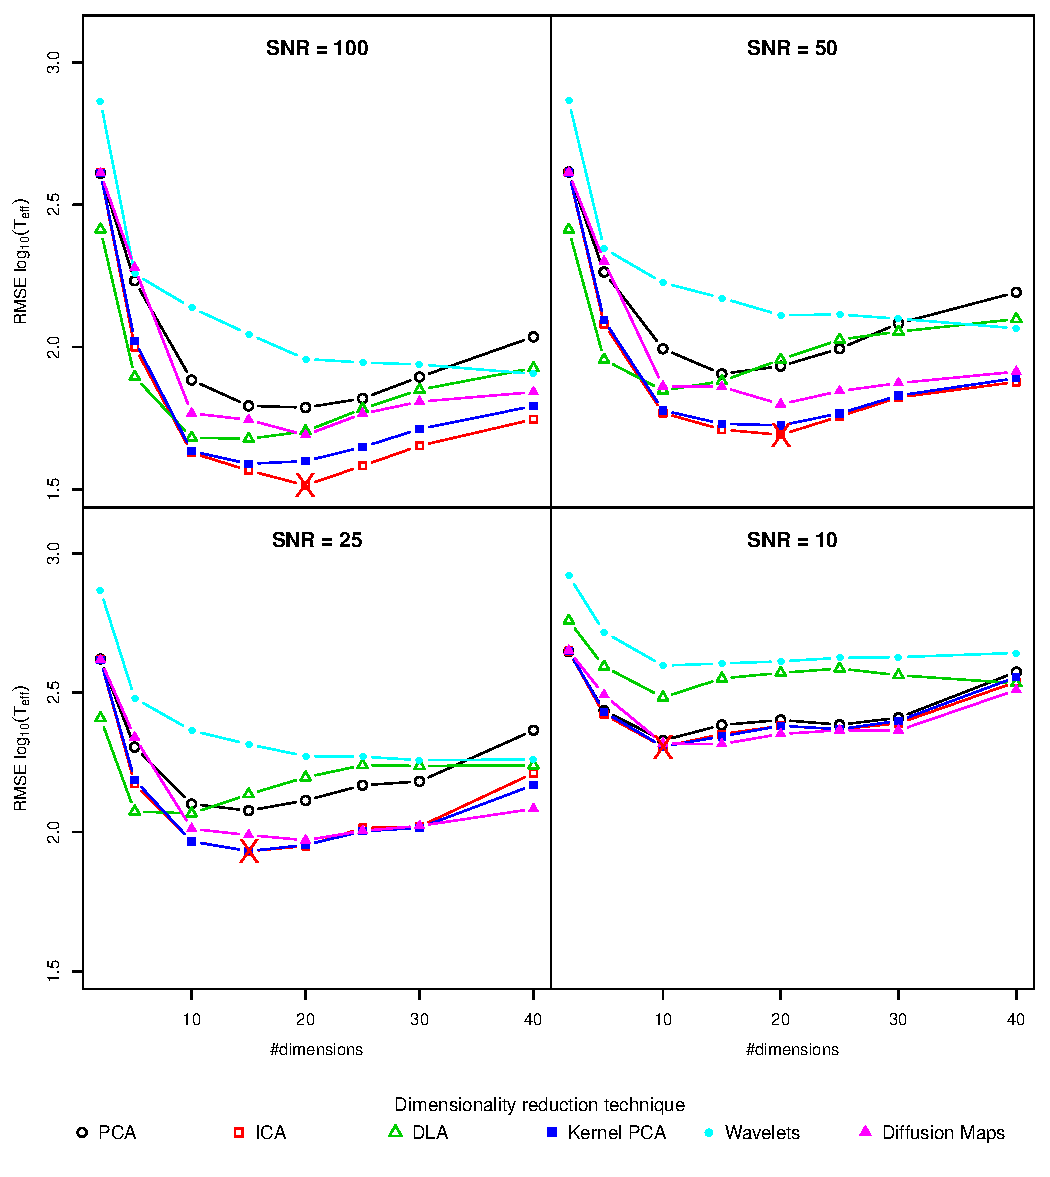
\includegraphics[width=\textwidth]{flamesHR21_Teff_log_BestSVM_N-RMSE_test.pdf}
\caption{Temperature estimation errors as a function of the number of
  dimensions used for data compression, for noisy synthetic
  spectra from the nominal GIRAFFE HR21 setup.}
\label{fig:02hr21}
\end{figure*}


\begin{table}
\centering
\caption{RMSE on the evaluation set of 2986 spectra for the best SVM trained models (HR21).}
\label{tab:hr21}
%\resizebox{0.99\textwidth}{!}{%
\begin{tabular}{l c c c}
\hline
\multirow{2}{*}{\textbf{SNR}} & \multirow{2}{*}{\textbf{Method}} & \multirow{2}{*}{\textbf{Nr. Dim.}} & {\bf RMSE}\\
 &  &  & \textbf{$T_{\rm eff}$ (K)}\\
\hline
$\infty$ & DLA & 15 & 12.58\\
100 & ICA & 20 & 32.69\\
50 & ICA & 20 & 49.18\\
25 & ICA & 15 & 82.36\\
10 & ICA & 10 & 202.39\\
\hline
%\multicolumn{6}{l}{$^1$ }\\
\end{tabular}
%}
\end{table}

%%%%%%%%%%%%%%%%%%%%%%%%%%%%%%%%%%%%%%%
\section{Optimal training set SNR}
\label{sec:comparison2}

In this Section we analyse the optimal match between the SNR of the training
set and that of the spectra for which the atmospheric parameter
predictions are needed (in the following, the evaluation set).

In order to analyse the dependence of the predicition accuracy with
the training set SNR, we generate 25 realisations of the noise for
each of the following 8 finite SNR levels: 150, 125, 100, 75, 50, 25,
10 and 5. We create the 25 noise realisation in order to estimate the
variance of the results and the significance of the differences. 
This amounts to $25\times 8=200$ datasets, plus the
noiseless dataset, all of which are compressed using ICA. The 20 
first independent components are retained for the subsequent 
regression stage. The choice of compression technique and target 
dimensionality was dictated by the results presented in the previous 
Section. For each of these datasets we trained an SVM
model to estimate each of the atmospheric parameters ($T_{\rm
  eff}$, log \textit{g}, [M/H] or $\left[ \alpha/Fe \right]$), and to 
assess the consistency of the results as the evaluation set SNR degrades. 
The model performances were evaluated using 10-fold cross validation 
as follows:

\begin{enumerate}
\item The noiseless dataset is replicated $25\times 8$ times: 25
  realisations of Gaussian white noise for each of the following SNRs:
  150, 125, 100, 75, 50, 25, 10, and 5. These 200 replicates together
  with the original noiseless dataset forms the basis for the next
  steps.
\item Each spectrum in each dataset is projected onto 20 independent
  components (as suggested by the experiments described in
  Section~\ref{sec:comparison1}).
\item Each of the 201 compressed datasets is then split into 10
  subsets or \textit{folds}. The splitting is unique for the 201
  datasets, which means that each spectrum belongs to the same fold
  across all 201 datasets.
\item \label{itemthree2} An SVM model is trained using 9 folds of each
  dataset (all characterized by the same SNR). This amounts to 201
  models.
\item \label{itemfour2} The model constructed in step \ref{itemthree2}
  is used to predict physical parameters for the tenth fold in all its
  201 versions. The RMSE is calculated independently for each value of
  the SNR and noise realisation.
\item \label{itemfive2} Steps \ref{itemthree2} to \ref{itemfour2} are
  repeated 10 times (using each time a different fold for evaluation)
  and the performance measure is calculated by averaging the values
  obtained in the loop.
\end{enumerate}

\subsection{Results}

Fig.~\ref{fig:snrtrain} shows the mean (averaged over the 25 noise
realisations) RMSE results and the 95\% confidence interval for the
mean as a function of the SNR of the evaluation set. The nine
different lines correspond to the SNR of the training set used to
generate both the projector and the atmospheric parameters predictor.
The main conclusions of the analysis can be summarised as follows.

The analysis yields the very important (albeit somehow predictable) 
consequence that models
trained with noise-free spectra are the worst choice for spectra 
with SNRs up 50/75, and are unnecessary for $T_{\rm eff}$, 
log \textit{g} and $\left[ \alpha/Fe \right]$ in contexts of higher 
SNRs. Only the [M/H] regression models slightly benefit from training 
with noiseless spectra if the evaluation spectra are in the SNR$\ge 50$ regime. 
The accuracy of the model trained with noise-free spectra degrades 
exponentially for SNR$<$50.

There are no large discrepancies amongst the estimations
obtained by applying the 25 models trained with a given SNR to
different noise realisations, which translates into small confidence
intervals and error bars in the plot. This is so even for the lowest
SNR tested (SNR=5).

For the effective temperature and metallicity estimation from 
evaluation spectra with SNR $ > 50$, there are minimal
differences in the precision achieved by models trained with spectra
of SNR$\ge 50$, while for evaluation sets with $50 \ge$ SNR $> 10$, 
the best accuracy is obtained with the model constructed from spectra 
with SNR of 50. For SNR lower than 10, the model with best generalisation
performance is that trained with SNR=10. Hence, two models suffice to 
obtain the best performance across the entire SNR range explored in 
this set of experiments: one trained with SNR=50 examples for evaluation 
spectra of any SNR above 10, and one trained with SNR = 10 examples 
for lower SNRs. 

Finally, only one ICA+SVM model trained with SNR=25 examples would be enough to
estimate the surface gravity for spectra of all SNRs with the best
performance (the SNR=50 model yielding similar although lower performances), 
and only one ICA+SVM model trained with SNR of 50 would be enough to
estimate the alpha to iron ratio for spectra of all SNRs.

\begin{figure*}
\centering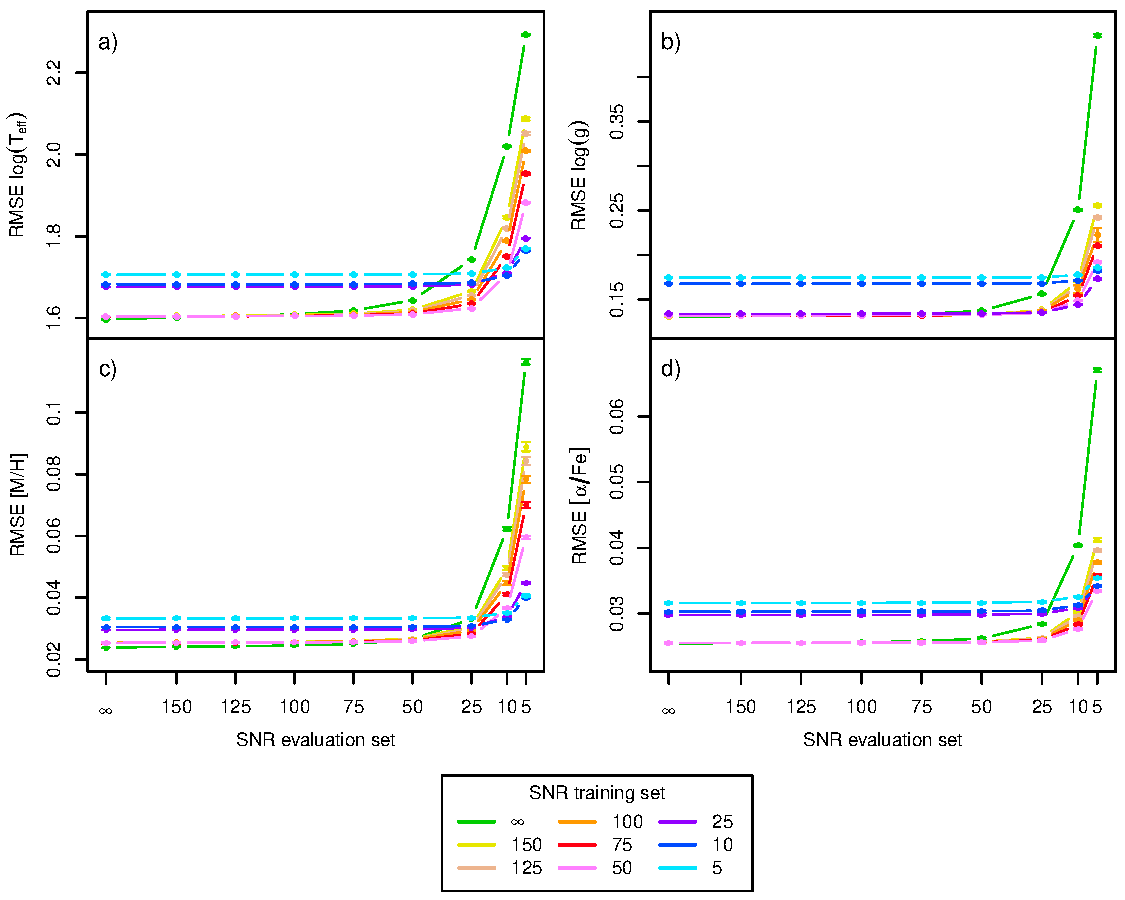
\includegraphics[width=\textwidth]{snr_errors_log_global_2x2.pdf}
\caption{Estimation errors as a function of the SNR of the evaluation
  set for $T_{\rm eff}$ (a), $\log(g)$ (b) and [M/H] (c) and
  $\left[ \alpha/Fe \right]$ (d). Each line corresponds to a model 
  trained with a specific SNR (nominal GIRAFFE HR10 setup).}
\label{fig:snrtrain}
\end{figure*}

As a summary, models trained with noiseless spectra are either 
catastrophic choices or just equivalent to other models. Moreover, 
there is no need to match the SNR of the training set to that of the 
real spectra because only two ICA+SVM models would be enough to 
estimate $T_{\rm eff}$ and [M/H] in all SNR regimes, and a single 
model is needed for the optimal prediction of surface gravities and 
alpha to iron ratios.

%%%%%%%%%%%%%%%%%%%%%%%%%%%%%%%%%%%%%%%%%%%%%%%
%%% HR21
\subsubsection{Application to the HR21 setup spectra}

The same evaluation procedure described above was applied to the 
HR21 setup spectra in order to check for the applicability of our 
conclusions in different wavelength ranges and coverages. Figure~\ref{fig:snrtrainhr21} 
shows the results obtained for the prediction of $T_{\rm eff}$.

\begin{figure}
	\centering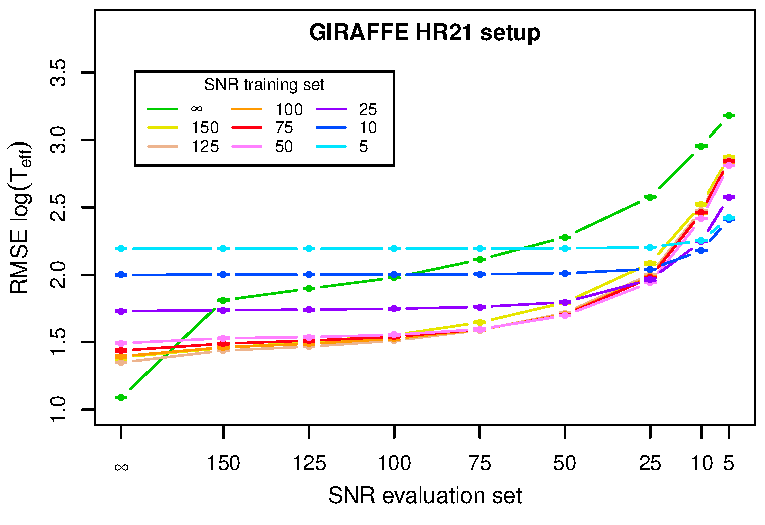
\includegraphics[width=\columnwidth]{snr_errors_log_global_HR21.pdf}
	\caption{Estimation errors as a function of the SNR of the HR21 evaluation 
		set for $T_{\rm eff}$. Each line corresponds 
		to a model trained with a specific SNR.}
	\label{fig:snrtrainhr21}
\end{figure}

Again, we observe that there is no need to match 
the SNR of the training set to that of the real spectra. Models 
trained with noise-free spectra are only adequate to 
estimate $T_{\rm eff}$ of noise-free spectra, and completely 
useless in any other SNR regime. This effect is much more evident 
here than in the case of the HR10 setup. 

It is also clear that again, if the evaluation spectra 
are in the SNR>25 regime, the $T_{\rm eff}$ 
regression models have to be trained with SNR$\ge$50 examples.
For evaluation spectra with SNR$\ge$100, the differences 
in the precision achieved by models trained with spectra of 
SNR$\le$50 are easier to notice than in the HR10 setup. There, the best 
option is one ICA+SVM model trained with SNR of 125.

In summary, our conclusions for the HR10 setup remain valid, except 
that a third model a model trained with SNR=125 examples would be marginally 
better than the SNR=50 one in the highest SNR regime (that is, above 100). 

%%%%%%%%%%%%%%%%%%%%%%%%%%%%%%%%%%%%%%%
\section{Training set density}
\label{sec:comparison3}

In this Section we evaluate the dependence of the regression 
RMSE with the training set density. In order to simplify the 
interpretation of the results, we restrict the problem to solar 
metallicities and alpha abundace ratios. This simplification 
reduces the set of available spectra from 8780 to only 137 
spectra in HR10 setup dataset with solar [M/H] and [alpha/Fe]. 
These 137 spectra are situated at the nodes of a regular 
grid except for a few gaps (see Fig. \ref{fig:gridModelos}) 
that were interpolated as a weighted bilinear combination four 
nearest neighbours in the space of physical parameters. Thereafter, 
succesive grid refinements were obtained by recursively interpolating 
spectra at intermediate points between grid nodes. These interpolated 
spectra were obtained again as weighted linear combinations of the 
bracketing spectra, with weights given by the inverse square of 
the normalized euclidean distance to the nearest neighbours.

A total of six grids of synthetic spectra with different grid densities were used to
train SVM models. The $T_{\rm eff}$ values varied between 4000 and
8000 K with step-sizes equal to 50, 62.5, 100, 125, 200, and 250 K. The other
grid parameters were established as follows: the log \textit{g} were
regularly sampled from 1 to 5 dex in steps of 0.5 dex and both [M/H] and $\left[
\alpha/Fe \right]$ were set equal to zero. Table~\ref{tab:grid} presents 
the step-sizes used in this study as well as the number of synthetic spectra available in each
grid.  In addition to this, noisy replicates of these grids were
generated for four different SNR levels (100, 50, 25, 10).


\begin{table}
\centering
\caption{Size of the new datasets computed with different grid densities.}
\label{tab:grid}
\begin{tabular}{c c}
\hline
\textbf{$T_{\rm eff}$ step-size (K)} & \textbf{Number of spectra} \\
\hline
50 & 679 \\
62.5 & 545 \\
100 & 343 \\
125 & 277 \\
200 & 175\\
250 & 143\\
\hline
\end{tabular}
\end{table}

We evaluated the performance of the SVM regression models using
10-fold cross validation. Figures \ref{fig:grid50} and
\ref{fig:grid10} present the $T_{\rm eff}$ estimation errors obtained
with the different grid densities and the two optimal training set
SNRs (50 and 10) found in the previous Section. Similar 
figures for SNR=25 and 100 are shown in Appendix \ref{a2}.

As expected, the estimation errors increase when the grid 
density decreases. We see how ICA remains as a winning 
alternative in this second scenario (a simplified training 
set with no variation in metallicity or $\left[ \alpha/Fe \right]$), 
where kernel PCA becomes non optimal and another linear 
technique (PCA) takes its place amongst the best performing 
techniques. 

The prevalence of our conclusion for ICA as a winning alternative 
regardless of the grid spacing is reassuring. However, the non linear 
version of PCA lost its place amongst the best 
performing compression techniques. It is 
evident from the comparison of Figs. \ref{fig:methodsnrTeff} and 
\ref{fig:grid50} that it is only at the largest grid spacings (250 K) 
that the non linear version of PCA performs better than the linear 
version (consistent with the results declared in Section 
\ref{sec:comparison1}), because the latter improves faster due to 
the grid refinement. It remains to be tested whether this faster 
decrease in the RMSE is due to the 
reduction in the training set complexity brought about by the removal 
of the non solar metallicities and $\left[ \alpha/Fe \right]$ ratios, 
or it is still present in the full space of four physical parameters. 
It is plausible that the simplification to solar abundances brings the 
distribution of examples in feature space closer to a gaussian distribution 
where indeed the first principal components are effectively more 
correlated with the effective temperature.

It is interesting to note that the (non linear) compression with 
Diffusion Maps benefits much less from the grid refinement than the 
linear compression techniques PCA and ICA. Given the high dimensionality 
of the input space, it may be the case that much finer grid spacings 
are needed for the benefits of Diffusion Maps to become apparent. More 
experiments are needed to confirm this hypothesis, but insofar as the 
grid spacings are constrained to the values tested here, Diffusion Maps 
remain suboptimal choices.

\begin{figure*}
\centering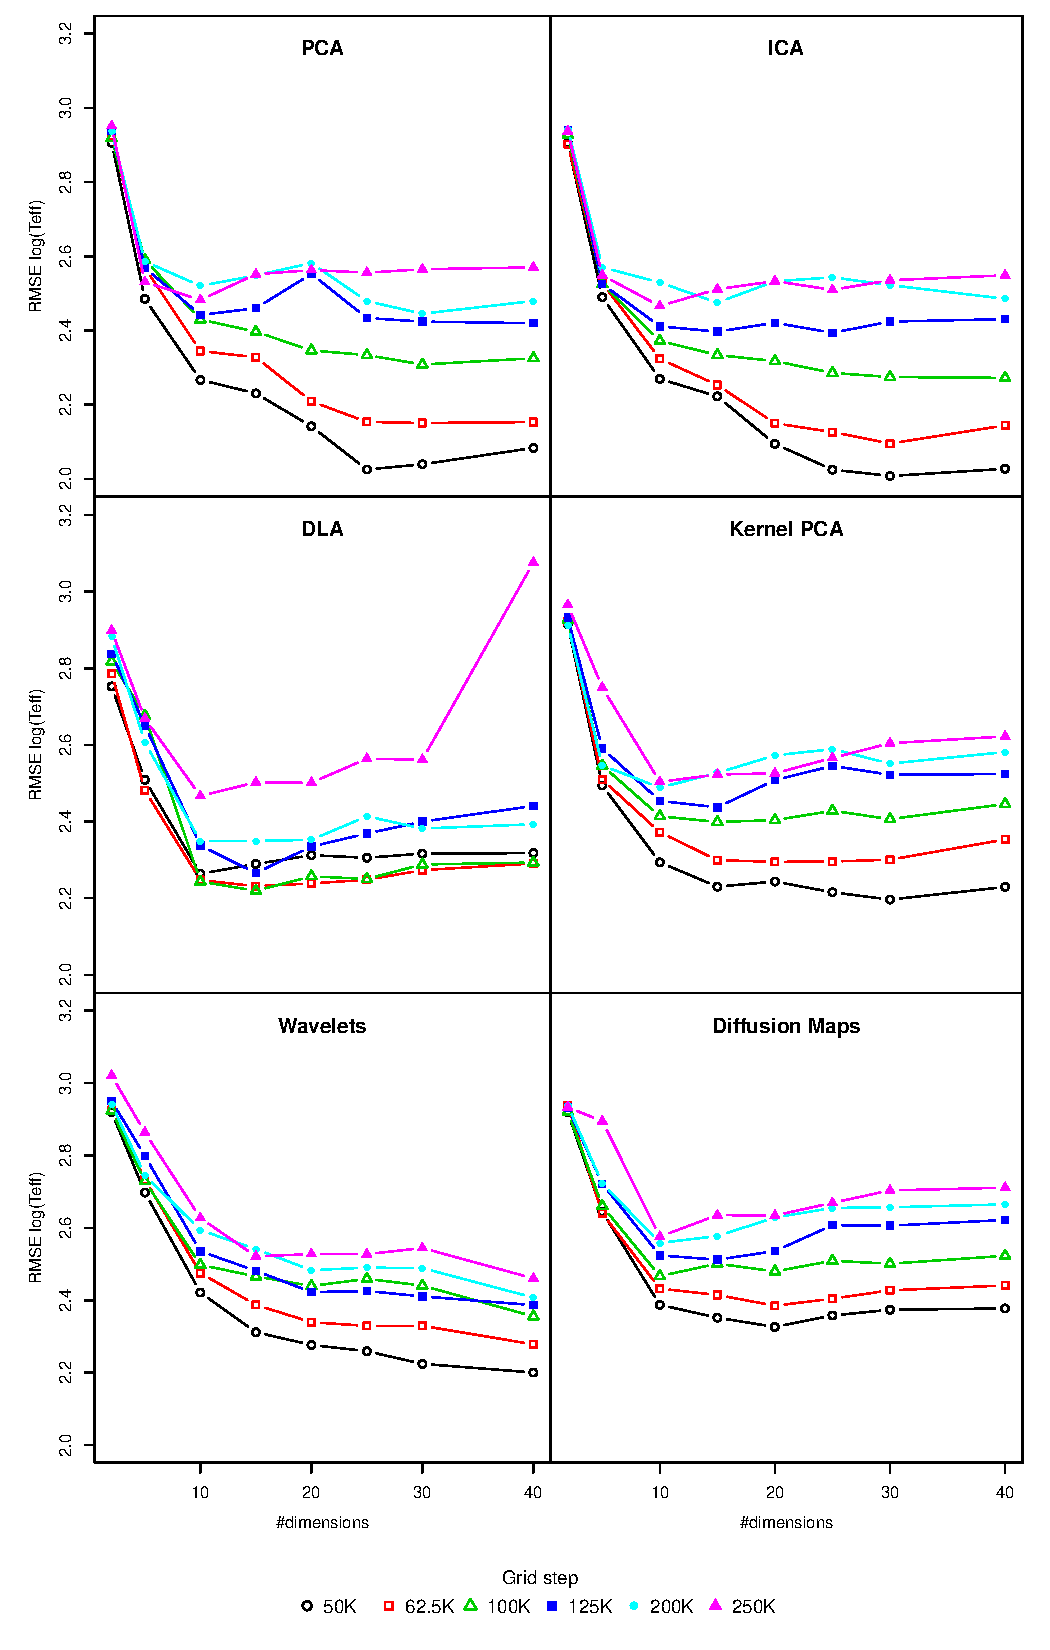
\includegraphics[width=\textwidth]{bestSVM_Teff_N-RMSE_HR10_snr=50_all.pdf}
\caption{Temperature estimation error against the number of dimensions
  used for data compression. Each line corresponds to a model trained
  with a specific grid step (SNR = 50)}
\label{fig:grid50}
\end{figure*}

\begin{figure*}
\centering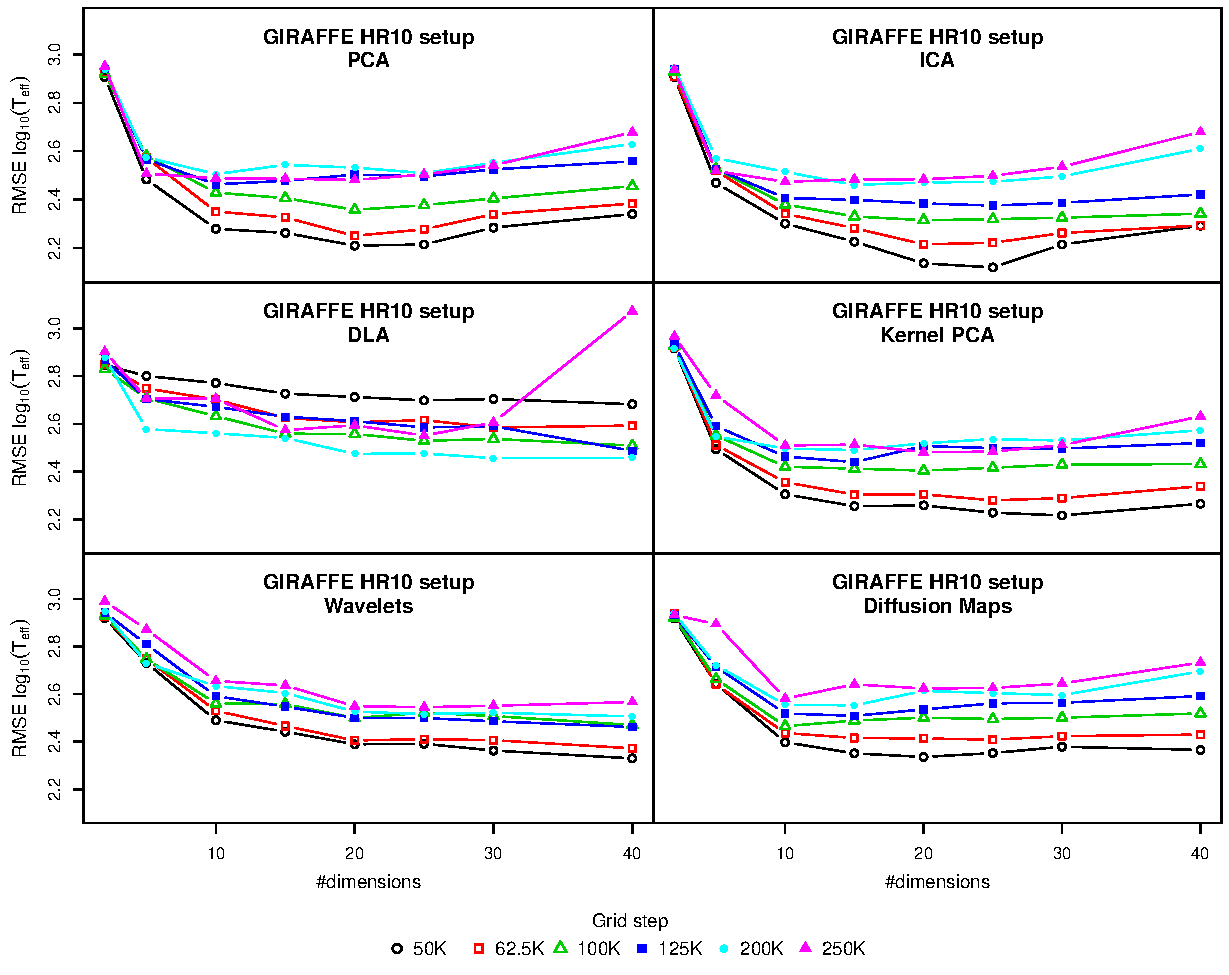
\includegraphics[width=\textwidth]{bestSVM_Teff_N-RMSE_HR10_snr=10_all.pdf}
\caption{Temperature estimation error against the number of dimensions
  used for data compression. Each line corresponds to a model trained
  with a specific grid step (SNR = 10)}
\label{fig:grid10}
\end{figure*}

\section{Conclusions}
\label{sec:conclusions}

In this work we have carried out a complete set of experiments to 
guide users of spectral archives to overcome the problems associated 
with the curse-of-dimensionality, when inferring 
astrophysical parameters from stellar spectra using standard machine 
learning algorithms. 

In Section \ref{sec:comparison1} we demostrate that, taken globally 
(that is, including the four stellar atmospheric parameters, a 
range of SNRs, and a range of compression ratios),
Independent Component Analysis outperforms all other techniques, followed  
by Kernel Principal Component Analysis. The comparative advantage of 
using ICA is clearer for the $T_{\rm eff}$ and $\left[ \alpha/Fe \right]$ 
regression models, and less evident for $\log g$ and [M/H]. Furthermore, 
we prove that this advantage holds too for a completely different wavelength range 
and a wavelength coverage twice as large. This is not enough to recommend 
ICA compression of high resolution spectra for any spectrograph observations, but it 
is a good indication that our results are not strongly dependent on the 
actual characteristics of the spectra. 

The conclusions drawn from the set of experiments described in Section \ref{sec:comparison1}
are tied to the restricted range of physical parameters, wavelengths,
and the spectral resolution of the datasets adopted (the HR 10 and 21 setups), but we hope that they
still hold for datasets of similar characteristics (different
wavelength ranges but similar resolutions and parameter subspaces). In
completely different scenarios such as the coolest regions of the
Hertzsprung-Russell diagram, where spectra are dominated by molecular
absoption bands, the validity of our results still remains to be proved.

In Section \ref{sec:comparison2} we show that there is no need to match 
the SNR of unlabelled spectra (the spectra for which we want to predict 
astrophysical parameters) with a regression model trained with the same SNR. 
On the contrary, only two models are needed to achieve optimal performance 
in $T_{\rm eff}$ and $\left[ \alpha/Fe \right]$ regression models (one trained 
with SNR=50 examples for SNR > 10 spectra and one trained with SNR=10 examples 
for the lowest SNR regime), and only one model is needed for the prediction 
of $\log g$ and [M/H] (trained with SNR=25 and 50 examples respectively). 
The $T_{\rm eff}$ result holds also for the HR21 setup regression, although the  
model trained with SNR=125 is marginally better than the SNR=50 one in the highest 
SNR regime above 100.

In Section \ref{sec:comparison3} we demostrate in a very simplified setup with 
no metallicity or alpha-enhancement effects incorporated in the training set,
the importance of dense training sets in reducing the cross-validation errors, 
even in the context of compressed data spaces. We emphasize that this is only 
applicable to cross-validation errors (that is, errors estimated from spectra 
entirely equivalent to those used for training). These cross-validation errors 
are often known as internal errors as they do not take into account systematic 
differences between the training and evaluation sets. In our case, we have used 
MARCS model atmospheres, not observed spectra of real stars. In practical 
applications of the results presented above, the mismatch between the training 
set and the observed spectra inevitably leads to additional errors.
It seems a reasonable working hypothesis to assume that there is a limit beyond 
which the total errors are dominated by this mismatch and further increasing the 
training grid density will not significantly decrease the total errors.  

Again, ICA turns out to be the best performing compression technique in the 
simplified experiments described in Section \ref{sec:comparison3}. The 
underlying assumptions of ICA may not be 
fulfilled to their full extent in the context of stellar 
spectra, but certainly we have reasonable hints that they 
apply, even if approximately. Our 
working hypothesis is that the independent components reflect 
groupings of spectral lines of various atomic elements with 
similar behaviour, such that the strengths and shapes of the 
lines pertaining to a given component respond in the same way 
to changes in the atmospheric parameters. Any such component 
would certainly have a non gaussian distribution across our 
training set (assumption one), albeit the fulfillment of the 
statistical independence assumption is, however, less clear 
under our interpretation of the ICA components. JADE maximizes 
non-gaussianity (rather than minimizing mutual information as 
in other flavours of ICA) via the fourth order moment of the 
distribution, and this turns out to result in the best projection 
amongst those tested in our regression models. This is certainly 
a result that holds for the synthetic spectra that constitute 
our working data set, but we have hints that this holds too for 
observed spectra \citep{2013A&A...550A.120S}.
 
There are other reasons that may limit the applicability of the results 
presented in this work. Extending the applicability analysis to prove our 
conclusions universally valid is beyond the scope of this article.

In the first place, we have used the most standard or general versions of 
the techniques evaluated here. In the case of wavelet compression, for example, 
there are approaches to coefficient shrinkage other than simply removing 
the smallest spatial scales. The bibliography is endless and it would be 
impossible to test each and every proposed variation of the techniques 
presented here. In any case, it is important to note that the validity of 
our conclusions is limited to the standard versions tested here. 

Another source of limitation is due to the use of a single regression model to 
assess the prediction errors. Again, Support Vector Machines and empirical 
risk minimization are very standard and robust statistical learning techniques 
amongst the top performing models for a very wide range of real life problems 
\citep{vanGestel2004}. Of course, the no-free-lunch theorem \citep[see][and 
references therein for a formal statement of the theorem]{Igel2005} always 
allows for the existence of algorithms that perform better than SVMs for this 
particular problem, but in the absence of free lunches, SVMs are a very 
reasonable choice and a good standard to measure the compression 
techniques.

Finally, we have focused our research in a battery of discriminative regression 
models where the {\it curse-of-dimensionality} may lead to severe problems. Forward 
models such as the {\it Cannon} \citep{2015ApJ...808...16N} are not affected by 
this {\it curse-of-dimensionality} but would certainly benefit from a reduction 
of the more than 80000 parameters needed to model each and every flux in the spectrum.

\section*{Acknowledgements}
This research was supported by the Spanish Ministry of Economy and
Competitiveness through grant AyA2011-24052.



%%%%%%%%%%%%%%%%%%%%%%%%%%%%%%%%%%%%%%%%%%%%%%%%%%

%%%%%%%%%%%%%%%%%%%% REFERENCES %%%%%%%%%%%%%%%%%%

% The best way to enter references is to use BibTeX:

\bibliographystyle{mnras}
\bibliography{references} % if your bibtex file is called example.bib

%%%%%%%%%%%%%%%%%%%%%%%%%%%%%%%%%%%%%%%%%%%%%%%%%%

%%%%%%%%%%%%%%%%% APPENDICES %%%%%%%%%%%%%%%%%%%%%

\appendix

\section{Regression errors for the GIRAFFE HR10 setup grouped by compression technique.}
\label{a1}
\begin{figure*}
\centering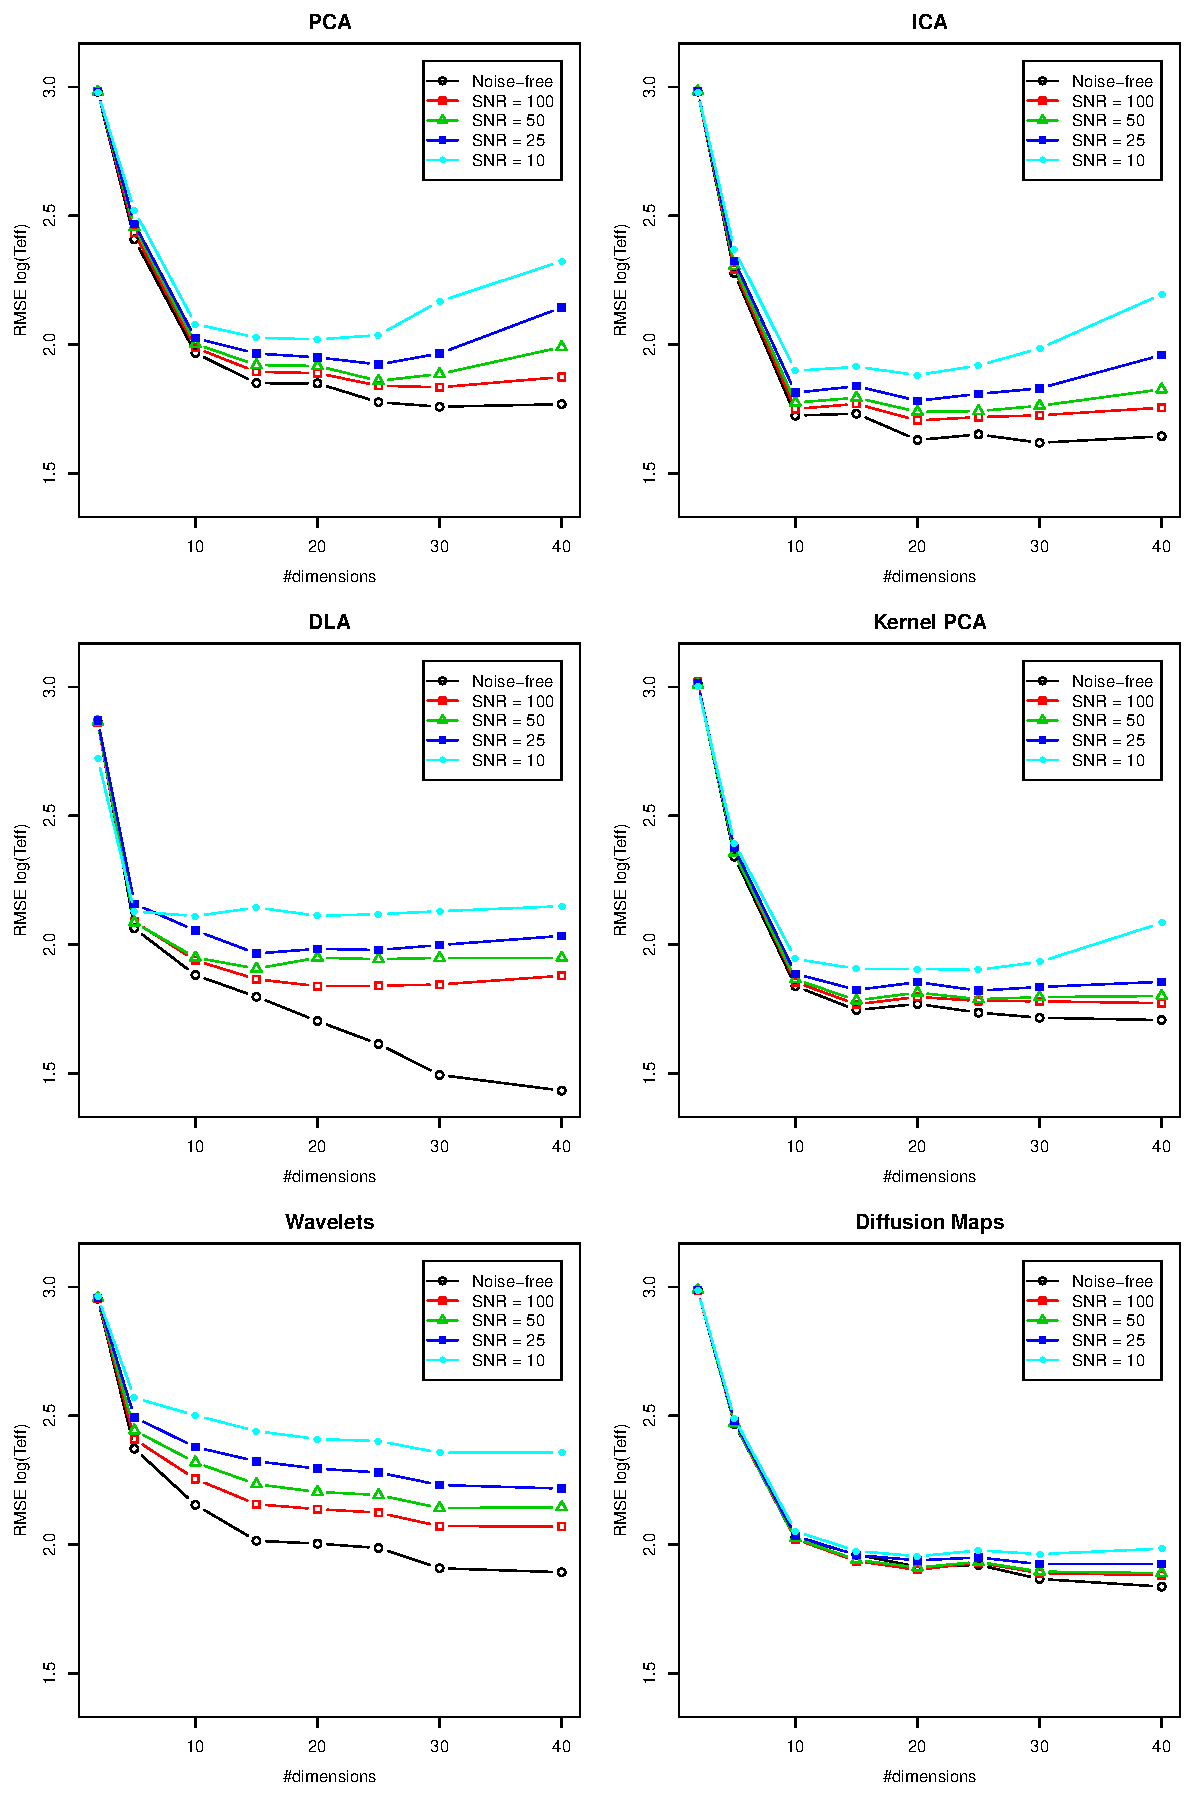
\includegraphics[width=\textwidth]{flamesHR10_Teff_log_BestSVM_N-SNR-RMSE_test.pdf}
\caption{Temperature estimation error against the number of dimensions
  used for data compression. Each line corresponds to a model trained
  with a specific SNR}
\label{fig:methodsnrTeff}
\end{figure*}

\begin{figure*}
\centering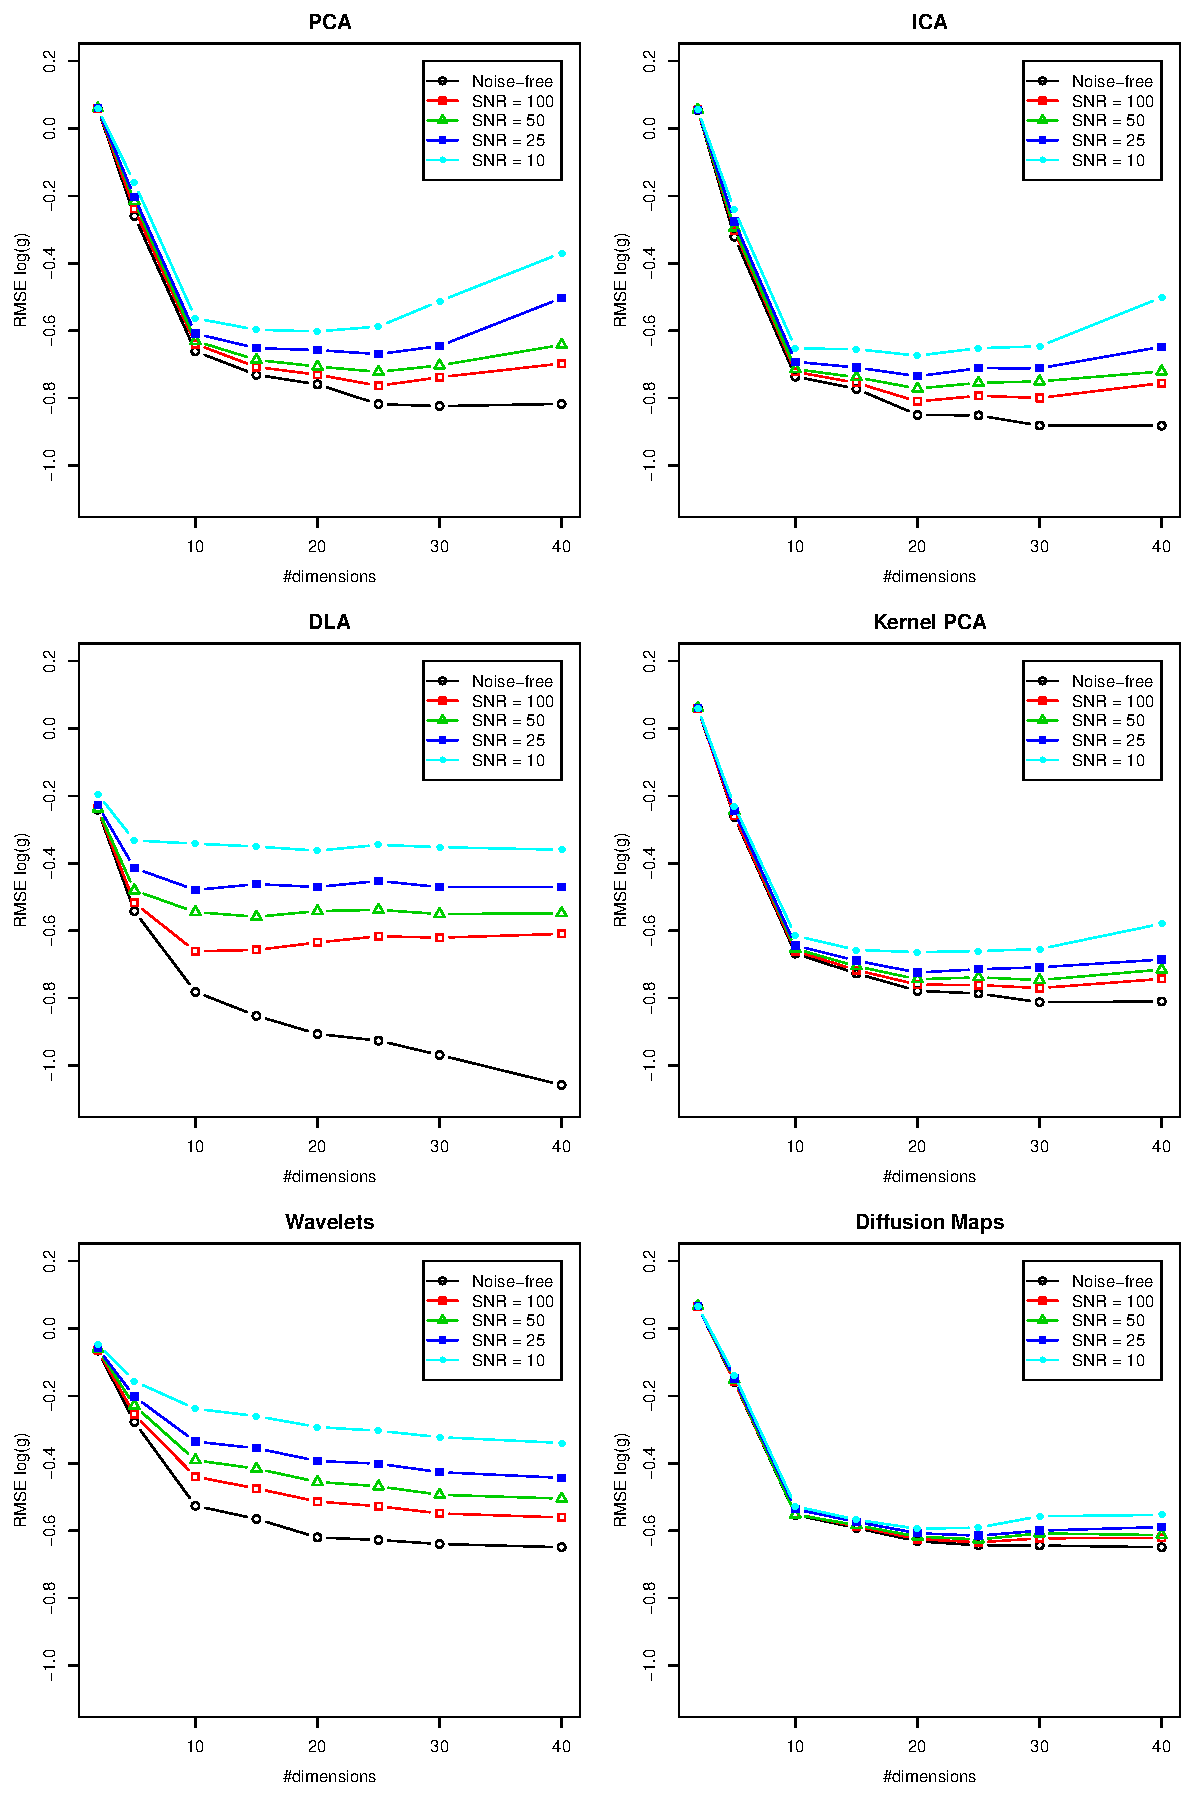
\includegraphics[width=\textwidth]{flamesHR10_Logg_log_BestSVM_N-SNR-RMSE_test.pdf}
\caption{Surface gravity estimation error against the number of dimensions
  used for data compression. Each line corresponds to a model trained
  with a specific SNR}
\label{fig:methodsnrLogg}
\end{figure*}

\begin{figure*}
\centering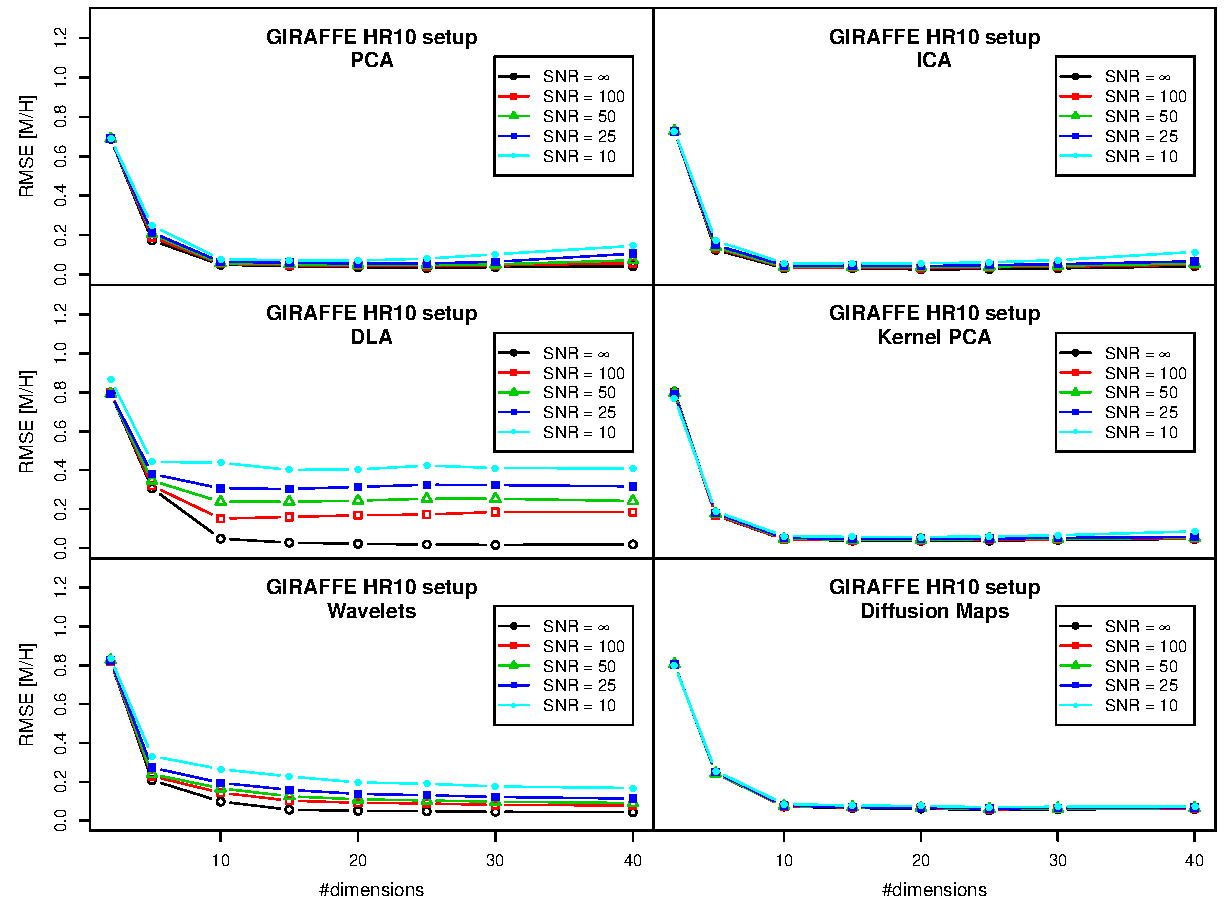
\includegraphics[width=\textwidth]{flamesHR10_Meta_log_BestSVM_N-SNR-RMSE_test.pdf}
\caption{Metallicity estimation error against the number of dimensions
  used for data compression. Each line corresponds to a model trained
  with a specific SNR}
\label{fig:methodsnrMeta}
\end{figure*}

\begin{figure*}
\centering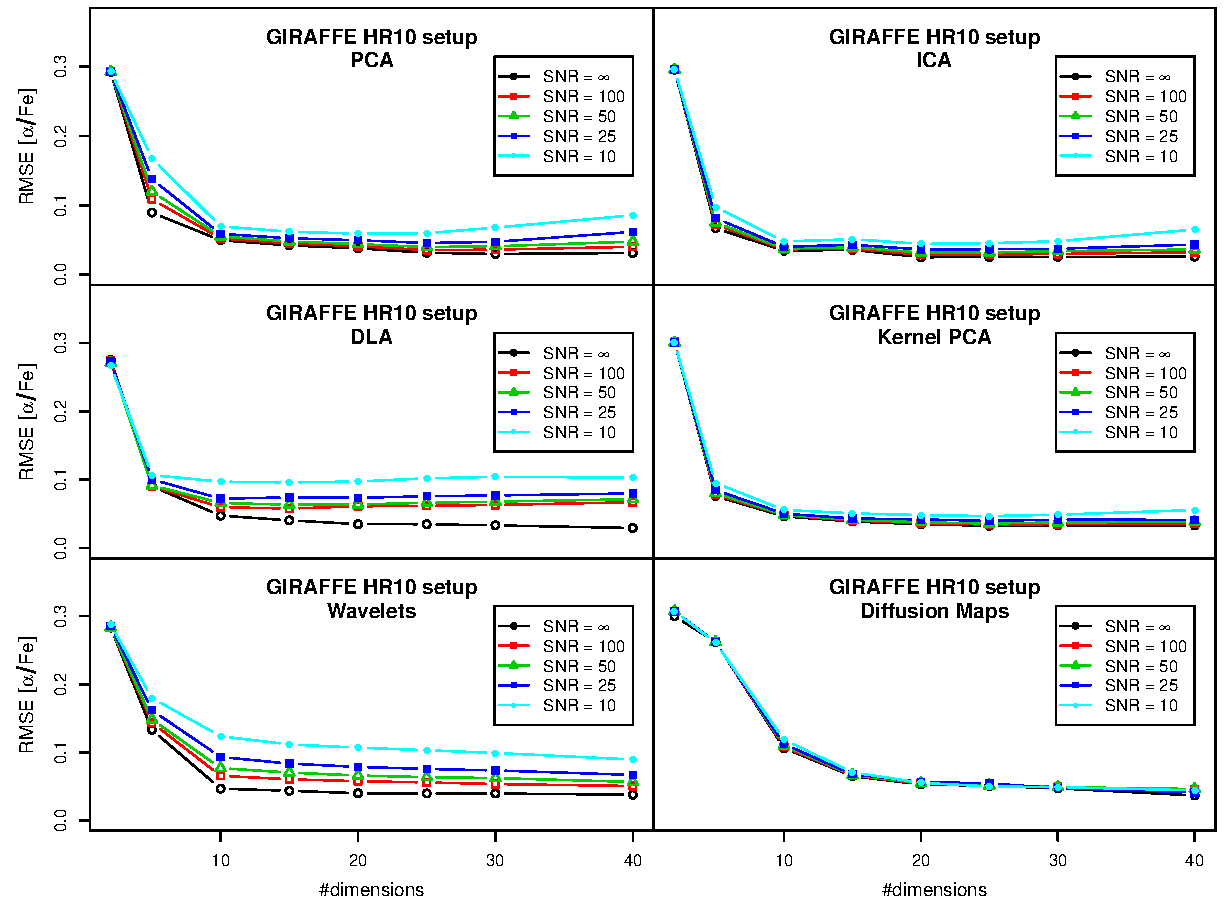
\includegraphics[width=\textwidth]{flamesHR10_AlFe_log_BestSVM_N-SNR-RMSE_test.pdf}
\caption{$\left[ \alpha/Fe \right]$ estimation error against the number of dimensions
  used for data compression. Each line corresponds to a model trained
  with a specific SNR}
\label{fig:methodsnrAlpha}
\end{figure*}

\section{Effective temperature regression errors as a function of the grid spacing and 
	grouped by compression technique for SNR=25 and 100}
\label{a2}

\begin{figure*}
\centering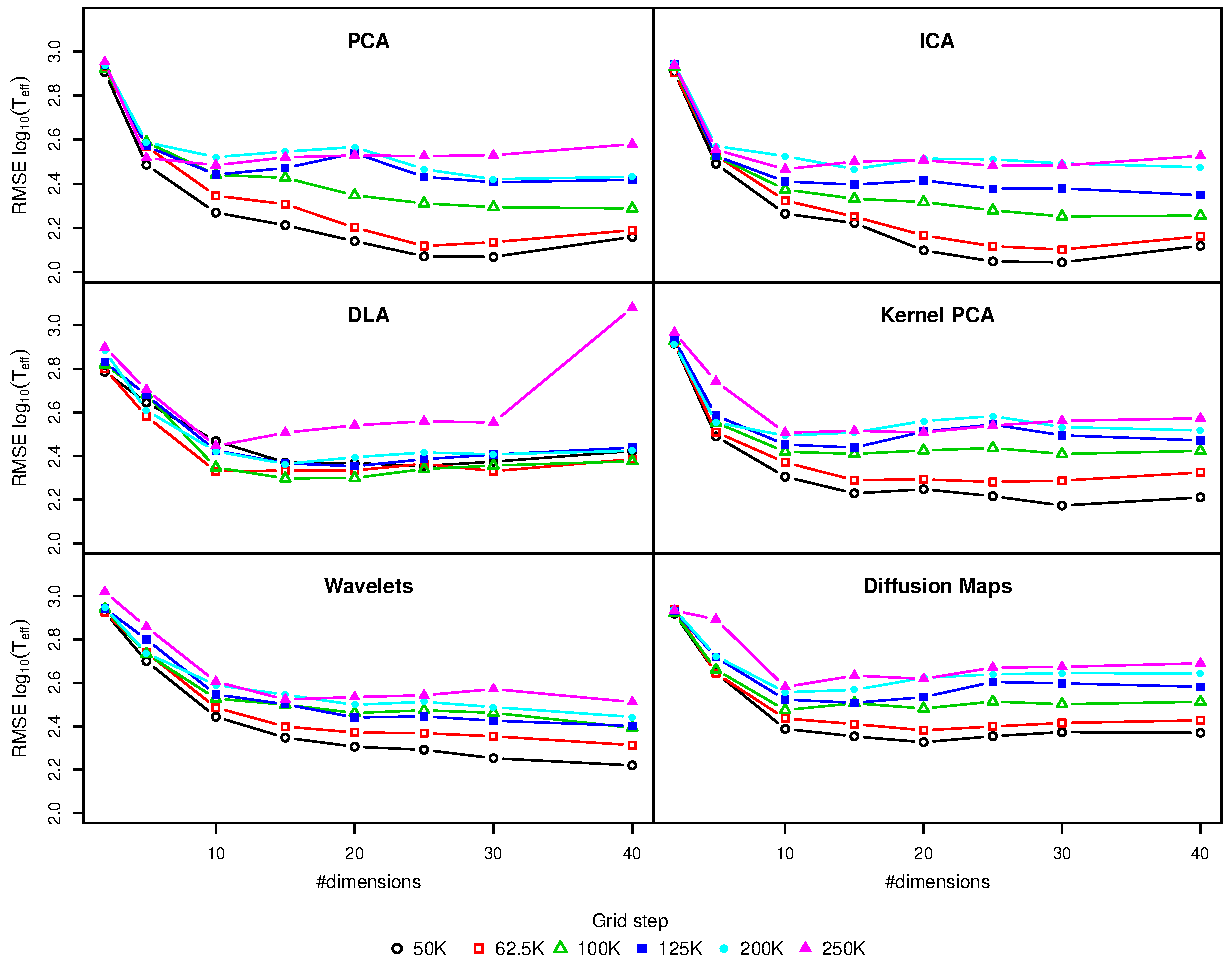
\includegraphics[width=\textwidth]{bestSVM_Teff_N-RMSE_HR10_snr=25_all.pdf}
\caption{Temperature estimation error against the number of dimensions
  used for data compression. Each line corresponds to a model trained
  with a specific grid step (SNR = 25)}
\label{fig:grid25}
\end{figure*}

\begin{figure*}
	\centering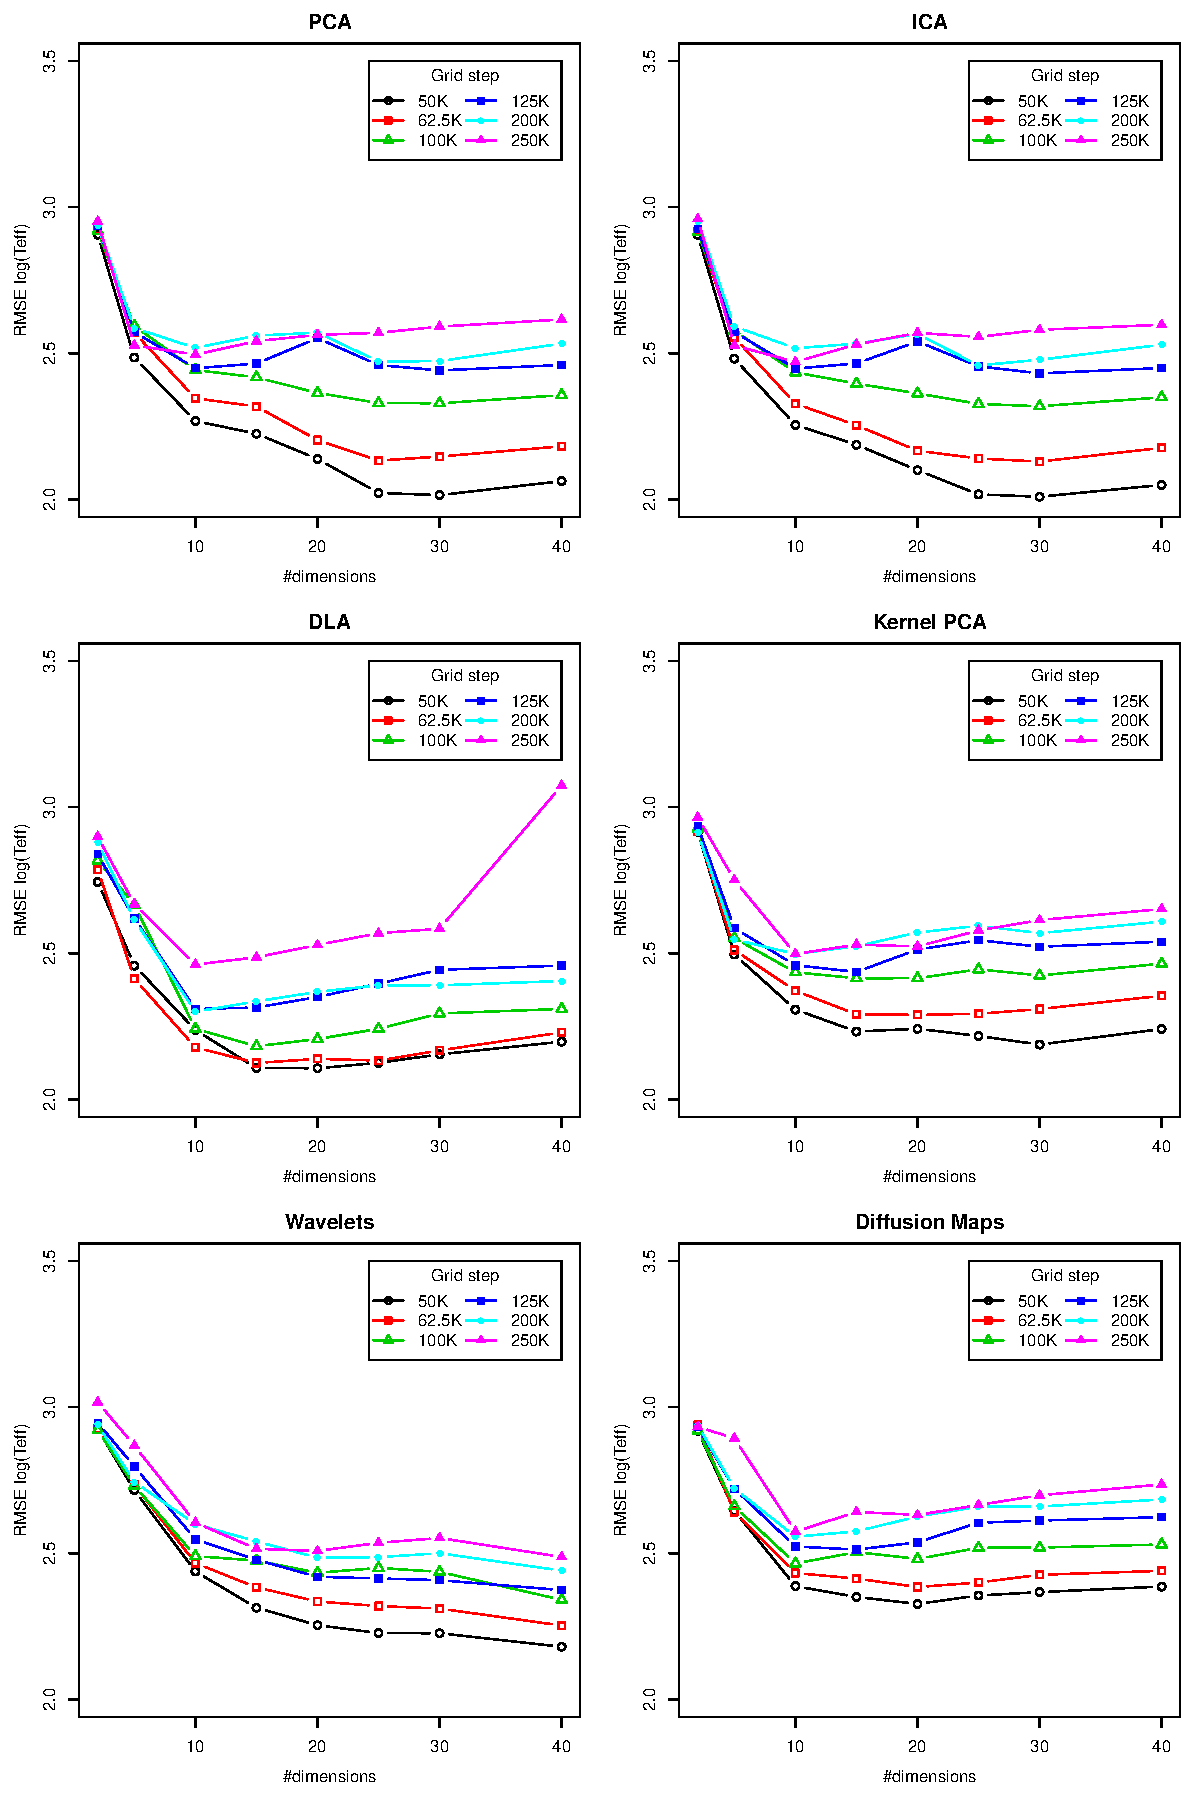
\includegraphics[width=\textwidth]{bestSVM_Teff_N-RMSE_HR10_snr=100_all.pdf}
	\caption{Temperature estimation error against the number of dimensions
		used for data compression. Each line corresponds to a model trained
		with a specific grid step (SNR = 100)}
	\label{fig:grid100}
\end{figure*}


%%%%%%%%%%%%%%%%%%%%%%%%%%%%%%%%%%%%%%%%%%%%%%%%%%


% Don't change these lines
\bsp	% typesetting comment
\label{lastpage}
\end{document}

% End of mnras_template.tex
